\chapter{Reinforcement Learning}
The robot controls its motors using artificial neural networks (ANN) and the deep deterministic policy gradient (DDPG) algorithm, developed by Lillicrap et al.\ \cite{lillicrap_2016}. The system runs in Python 3 \cite{python3}, leaning heavily on the TensorFlow library \cite{tensorflow} for artificial neural network instantiation, updating, and saving. The following sections briefly cover reinforcement learning (RL) techniques that form the foundation of DDPG. It is worth noting that Sutton's introductory book on RL provides excellent background on many of the following algorithms and more \cite{sutton_2017}.

\section{Reinforcement Learning Background}
Reinforcement learning (RL) is a subset of machine learning that aims to solve control and action selection problems rather than to perform classification or data clustering. Most reinforcement learning problems involve six main elements: an actor, the environment, rewards, a policy, a value function, and sometimes a model. An actor (sometimes called an agent) takes actions in an environment which returns a state and reward, illustrated in Figure \ref{fig:actor_env_loop}. The actor's primary goal is to maximize the accumulated reward received from the environment. A policy determines which actions the actor takes given the current state and can be considered a mapping from state to action. The value function indicates the long-term reward expected from a state so even if a state only has a small immediate reward, it may possess high value since it leads to high reward states. Some algorithms involve a model of the environment, allowing prediction of the next state from the current state and action. Table \ref{tab:rl_defs} summarizes some common terms and definitions used in the reinforcement learning literature.
\begin{figure}[H]   % [h] means here
	\centering 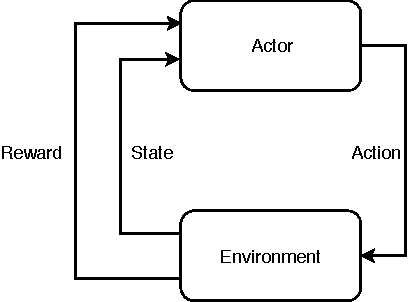
\includegraphics[width=3in, height=3.85in, keepaspectratio]{figures/actor_env_loop.pdf}
	\caption{Actor-Environment Feedback Loop}\label{fig:actor_env_loop}
\end{figure}
Actors strive to maximize the long-term discounted reward, $G_t$, where the subscript $t$ denotes the time step \cite{sutton_2017}. In RL problems with a definitive end (denoted by $t=T$) such as a game of chess, $G_t$ is finite and can be calculated simply as the sum of all future rewards (\ref{eq:Gt_simple}). 
\begin{equation}
	\label{eq:Gt_simple}
	G_t=R_{t+1}+R_{t+2}+\dots + R_{T}=\sum_{k=t}^{T-1} R_{k+1}
\end{equation}
However, continuous problems such as maintaining the temperature of a refrigerator have no maximum time step and therefore, a possibly infinite $G_t$. Shown in Equation \ref{eq:Gt_discount}, the introduction of a discount factor, $\gamma$, makes such a situation manageable. The discount factor weights the worth of future rewards exponentially by their distance into the future and ranges from 0--1 where 0 completely devalues future rewards while a discount factor of 1 weights all future rewards equally. In practice, the discount factor is less than 1 in order to allow $G_t$ to converge \cite{sutton_2017}. The discount factor can be considered a knob that sets the algorithm's outlook between myopic (short-sighted, only values immediate rewards) and far-sighted (willing to sacrifice immediate reward for greater long-term return).
\begin{equation}
\label{eq:Gt_discount}
	G_t=R_{t+1}+\gamma R_{t+2}+\gamma^2 R_{t+3} + \dots = \sum_{k=0}^{\infty} \gamma^k R_{t+k+1}
\end{equation}

The value function is the expected long-term reward as function of the state under a certain policy $\pi$ (\ref{eq:value_func}). The $\mathbb{E}_\pi$ operator evaluates the expected value provided the actor follows policy $\pi$.
\begin{equation}
	\label{eq:value_func}
	V_\pi(s)=\mathbb{E}_\pi [G_t | S_t =s]
\end{equation}

Core to many RL algorithms, the Q-function or action-value function is the expected long-term reward as a function of the state \textbf{and action} under a certain policy $\pi$ (\ref{eq:q_func}). The important distinction from the value function is dependency on the action. 
\begin{equation}
	\label{eq:q_func}
	Q_\pi(s,a)=\mathbb{E}_\pi [G_t | S_t =s, A_t=a]
\end{equation}

\LTXtable{\textwidth}{tables/tab_rl_defs.tex}

\section{Reinforcement Learning Algorithms}
Many reinforcement learning algorithms have been applied to control including Q-Learning, State-Action-Reward-State-Action (SARSA), deep Q-network (DQN), policy gradients (PG), deep policy gradients (DPG), and deep deterministic policy gradients (DDPG), among others \cite{sutton_2017}\cite{sutton_policygrad}\cite{silver_2017}\cite{silver_lever_heess_degris_wierstra_riedmiller}\cite{lillicrap_2016}. Note that these methods differ from evolutionary algorithms in that they actively learn as they interact with the environment.

RL algorithms can be classified by their use of models (model-based vs.\ model-free) and actor policy (on-policy vs.\ off-policy) \cite{sutton_2017}. Model-based strategies first develop a model of the environment and then use a planning algorithm along with the model to create a controller while model-free algorithms forgo the model entirely.

On-policy algorithms learn the policy followed by the actor while off-policy strategies learn a policy different from the one followed by the actor. For example, in Q-learning, the Q-function learns a greedy policy regardless of which policy the actor is following \cite{sutton_2017}. Various policies exist but the most commonly referred to in the literature include optimal, greedy, $\epsilon$-greedy, and random. The optimal policy $\pi_*$, by definition, produces greater value for every possible state than any other policy $\pi$, expressed in (\ref{eq:optimalpol}) where $\mathcal{S}$ is the set of all possible states. An actor using the greedy policy always takes the action with the highest value or Q-value depending on implementation. The $\epsilon$-greedy policy tells an actor to pick the greedy action with probability $1-\epsilon$ and a random action with probability $\epsilon$. Finally, an actor under the random policy always takes random actions.
\begin{equation}
	\label{eq:optimalpol}
v_{\pi_*}(s) \geq v_{\pi}(s), \forall s \in \mathcal{S}
\end{equation}

\subsection{Q-Learning}
Q-Learning is an off-model, off-policy algorithm that estimates the Q-function of the environment. The Q-function represents the "quality" of every possible action in every possible state. For example, imagine a game of tic-tac-toe as shown in Figure \ref{fig:tictactoe}. Each of the nine spaces can take one of three values (blank, X, or O) so the game has $3^9=19,683$ possible states (although some states are not achievable as the game would end once a player gets three in a row). Given a particular state, the Q-function returns the quality, i.e.\ predicted goodness, of each possible action the player could take. Therefore, the optimal action to take is simply the one with the highest Q-value. 
\begin{figure}[H]   % [h] means here
	\centering 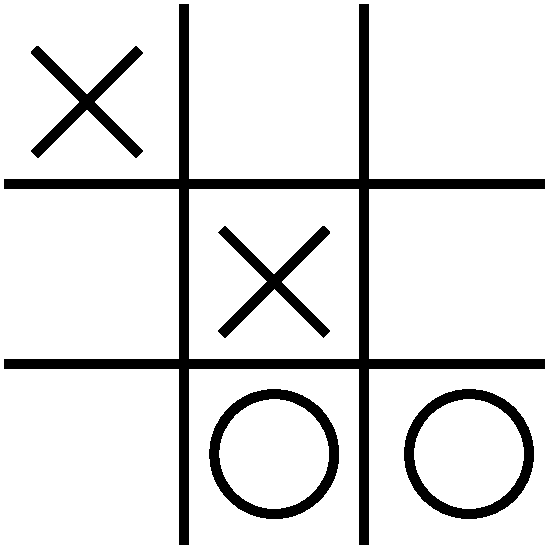
\includegraphics[width=2in, height=3.85in, keepaspectratio]{figures/tictactoe.pdf}
	\caption{A Game of Tic Tac Toe}\label{fig:tictactoe}
\end{figure}

Clearly, the Q-function always exists but not necessarily in an analytic or obvious form. So-called tabular Q-learning methods use a 2-D matrix to represent the Q-function with rows for all possible states and columns for all possible actions \cite{mccullock}. The table is initialized with guesses (possibly randomly or with all elements set to 0) and iteratively updated to approximate the true Q-function using the Bellman equation (\ref{eq:bellman}).
\begin{equation}
	\label{eq:bellman}
	Q(s,a)=R(s) + \gamma (\text{max}_{a'}(Q(s',a')))
\end{equation}

To improve convergence, Equation \ref{eq:bellman} is modified to include the learning rate $\alpha$. The pseudocode for Q-learning presented by Sutton is reproduced in Table \ref{tab:qlearning_pseudo}. The $\text{max}_{a'}()$ operator maximizes its argument with respect to $a'$.
\begin{table}[h]
	\caption{Q-Learning Pseudocode}  \label{tab:qlearning_pseudo}
	\begin{tabular}{|p{0.9\linewidth}|}\hline % or any other width
		Initialize $Q(s,a)$ arbitrarily. \\
		Repeat (for each episode): \\
		\qquad Initialize $s$\\
		\qquad Repeat (for each step of episode):\\
		\qquad \qquad Choose $a$ from $s$ using policy derived from $Q$ (e.g., $\epsilon$-greedy)\\
		\qquad \qquad Take action $a$, observe $r$, $s'$\\
		\qquad \qquad $Q(s,a)\gets (1-\alpha)Q(s,a) + \alpha [r + \gamma \text{max}_{a'}Q(s',a')]$\\
		\qquad \qquad $s \gets s';$\\
		\qquad until $s$ is terminal \\
		\hline
	\end{tabular}
\end{table}

Notice the algorithm updates the Q-value, $Q(s,a)$, from the Q-value of the next state and greedy policy action, $\text{max}_{a'}Q(s',a')$, regardless of the policy and action taken by the actor. This characteristic makes Q-learning an off-policy algorithm. The Q-value for a particular state and action only updates when the actor visits said state and action so the actor must still explore (i.e.\ not always take greedy actions) for Q-learning to converge.

Clearly, the tabular Q method quickly becomes unfeasible for more complex problems, especially when the states or actions become continuous rather than discrete. When the action or state spaces are continuous, the algorithm must discretize them, forcing a tradeoff between resolution and tractability. For the tic-tac-toe example, the table would be 19,683 rows by 9 columns for a total of 177,147 Q-values while the Q-value table for a game of chess would possess more elements than there are atoms in the known universe.

\subsection{State-Action-Reward-State-Action (SARSA)}
SARSA is an on-policy algorithm which shares many characteristics with Q-learning. The name comes from the fact that the Q update equation uses the current \textbf{s}tate and \textbf{a}ction as well as the next \textbf{r}eward, \textbf{s}tate, and \textbf{a}ction. The pseudocode for SARSA presented by Sutton is reproduced in Table \ref{tab:sarsa}:
\begin{table}[h]
	\caption{SARSA Pseudocode}  \label{tab:sarsa}
	\begin{tabular}{|p{0.9\linewidth}|}\hline % or any other width
		Initialize $Q(s,a)$ arbitrarily. \\
		Repeat (for each episode): \\
		\qquad Initialize $s$\\
		\qquad Choose $a$ from $s$ using policy derived from $Q$ (e.g., $\epsilon$-greedy)\\
		\qquad Repeat (for each step of episode):\\
		\qquad \qquad Take action $a$, observe $r$, $s'$\\
		\qquad \qquad Choose $a'$ from $s'$ using policy derived from $Q$ (e.g., $\epsilon$-greedy)\\
		\qquad \qquad $	Q(s,a)\gets (1-\alpha)Q(s,a) + \alpha [r + \gamma Q(s',a')]$\\
		\qquad \qquad $s \gets s'; a \gets a'$;\\
		\qquad until $s$ is terminal \\
		\hline
	\end{tabular}
\end{table}

Unlike Q-learning, SARSA updates Q-values from the next state and next action $Q(s',a')$, making it an on-policy strategy. Like Q-learning, the actor must take exploratory actions for the algorithm to update Q at all states and actions and achieve convergence.

\subsection{Deep Q Network (DQN)}
Deep Q Networks, developed by Mnih et al. \cite{Mnih_2015}, aim to solve two significant problem with Q-learning: the inability to handle situations with large state and action spaces and the inability to generalize learnings to new situations \cite{sutton_policygrad}. As mentioned previously, maintaining Q-values for the entire state and action space of a complex problem requires enormous memory. The second problem has to do with how the Q-value table updates. In both Q-learning and SARSA, the algorithms iteratively update Q-values for visited (state, action) pairs. However, to fully update the Q-value table means exploring every possible state and action combination multiple times, a non-trivial task. In other words, the algorithms cannot provide reasonable Q-value estimates for unvisited situations.

To overcome these limitations, DQN replaces the tabular Q concept with an artificial neural network (ANN) where the inputs are the state and action and the output is the Q-value. The Q-network is denoted as $Q(s,a;\theta_i)$ where $\theta_i$ represents the network weights. The loss function (\ref{eq:dqn_loss_func}) is the squared error between the Q-network output and the "target Q-value" as defined by the Bellman equation, $y_j = r + \gamma \text{max}_{a'}Q(s', a';\theta^-_i)$  \cite{Mnih_2015}. For complete clarity, $Q(s,a;\theta^-_i)$ represents an identical but separate copy of Q-network $Q(s,a;\theta_i)$ except with weights $\theta^-_i$ from a previous iteration, explained later.
\begin{equation}
	\label{eq:dqn_loss_func}
L_i(\theta_i) = (r + \gamma \text{max}_{a'}Q(s', a';\theta^-_i)-Q(s,a;\theta_i))^2
\end{equation}

To assist DQN training, Mnih et al.\ used a technique called experience replay \cite{Mnih_2015} As the actor explores within environment, the algorithm records transitions consisting of the current state, action taken, reward, and next state at each time step into a so-called experience replay buffer. After collecting a minimum number of experiences, the artificial neural network trains from data sampled randomly from the buffer, hence the name "experience replay". The technique removes time correlations in the training data, improving convergence, and also allows experience reuse, advantageous when obtaining data is difficult or costly.

The second technique Mnih et al.\ used to counter training instability involves generating target Q-values, $y_j$, from an identical but separate ANN, called the target Q-network $\hat{Q}$ with weights $\theta^-_i$. In effect, this creates a time delay between when the weights of $Q$ are updated and when those updates affect the policy and target Q-network, reducing the likelihood of policy instability. 

For example, using a 64 transition mini-batch, the network randomly samples 64 transitions from the experience replay buffer and trains the network $Q$ with 64 iterations as in \ref{eq:dqn_loss_func}. After, the target network $\hat{Q}$ clones the weights $\theta_i$ from $Q$ and the process repeats.

DQN replaced the tabular Q with an artificial neural network to solve RL problems with large Q spaces. However, the policy still uses a discrete action space, posing a problem for situations requiring continuously variable actions. For example, a system with five actions discretized into only four bits each already produces 32,768 different actions. Policy gradient methods can overcome this limitation.

\subsection{Stochastic Policy Gradient Method}
Q-Learning, SARSA, and DQN are value-based methods as they rely on finding the environment's underlying Q-function and produce a policy to maximize Q. Policy gradient methods find the optimal policy directly which makes them policy-based strategies \cite{sutton_policygrad}. In fact, DeepMind's AlphaGo famously defeated grandmaster Go player Fan Hui in 2015 and Lee Sedol in 2016 using an algorithm incorporating a policy gradient method, definitively proving its viability \cite{silver_2017}.

The underlying premise of stochastic policy gradients is simple: get a state, take a particular action with probability $P(a)$, and record the reward. If the reward is "good", increase the probability of taking that action or decrease it if the reward is "bad". Note that the terms "good" and "bad" are intentionally vague as to not constrain them to one particular interpretation. After many iterations, the actor will most likely take actions that produce good rewards. But of course, not all is so simple. Much like the so-called "butterfly effect", a single action can cascade into a multitude of unknown futures meaning the worth of a particular action cannot be determined by the immediate reward produced \cite{Lorenz_1963}. 

Instead, the rewards are accumulated for a long period in episodes, at the end of which actions are judged based on the total reward. Now, a different issue arises: the credit assignment problem \cite{fu_2008}. If an episode contains 1,000 actions, which ones ultimately produced the good reward and which were inconsequential or detrimental? Rather than determining the individual actions responsible, the algorithm deems all actions in an episode culpable so if the episode outcome is good, all actions taken become more likely and if not, the inverse occurs \cite{karpathy_2016}. Like AlphaGo, many policy gradient implementations use an artificial neural network where the inputs are states and outputs are action probabilities \cite{silver_2017}. Therefore, the act of making actions more or less probable is carried out with the standard back-propagation algorithm where the gradient is adjusted by normalized episodic reward \cite{karpathy_2016}.
%A more concrete implementation is shown below in pseudocode where $P(s,a,\theta)$ represents the parametrized probability of action $a$ in state $s$ for all possible states and actions, $\theta$ represents the parameters controlling the probability distribution:
%\begin{center} \begin{tabular}{|p{0.9\linewidth}|}\hline % or any other width
%Initialize $P(s,a,\theta)$ arbitrarily. \\
%Repeat until satisfactory performance: \\
%\quad Policy rollout n times (typ. 20 to 100): \\
%\quad \quad Initialize $s$\\
%\quad \quad Repeat (for each step of episode):\\
%\quad \quad \quad Stochastically choose $a$ from $s$ using policy derived from $P(s,a,\theta)$\\
%\quad \quad \quad Take action $a$, observe $s'$, accumulate $r$\\
%\quad \quad \quad $s \gets s'$;\\
%\quad \quad until $s$ is terminal \\
%\quad Normalize the $r$ from n policy rollouts. \\
%\quad 
%\hline
%\end{tabular} \end{center}

\subsection{Deterministic Policy Gradient Method (DPG)}
The deterministic policy gradient method (DPG), developed by Silver et al., shares the same foundation as stochastic policy gradients, but instead of representing the policy as a probability distribution, the policy deterministically chooses actions from the given states \cite{silver_lever_heess_degris_wierstra_riedmiller}. Silver et al.\ have shown that the DPG is actually a limiting case of stochastic policy gradients where the policy distribution variance is 0. Another key difference is that while the stochastic policy gradient integrates over the state and action spaces, the DPG only integrates over the state space. Consequently, the stochastic case requires more samples to compute. Finally, the stochastic policy inherently chooses exploratory actions due to its probabilistic nature so Silver developed an off-policy learning algorithm using a stochastic policy to ensure sufficient exploration despite producing a deterministic policy.

\subsection{Deep Deterministic Policy Gradient (DDPG)}
The deep deterministic policy gradient algorithm, developed by Lillicrap et al., is a model-free, off-policy actor-critic strategy based on the Silver et al.'s DPG algorithm combined with learnings from Mnih et al.'s work on the DQN algorithm \cite{lillicrap_2016}\cite{Mnih_2015}\cite{silver_lever_heess_degris_wierstra_riedmiller}. DDPG improves on DPG by representing the actor policy with an ANN and applying the experience replay and target network techniques from DQN. 

Additionally, Lillicrap et al.\ adapted batch normalization from Ioffe's work to allow ANN hyper-parameter generalization for environments with features of varying magnitude \cite{2015arXiv150203167I}; each feature in a minibatch is normalized to unit mean and variance. In their implementation, batch normalization was applied to network inputs, all layers of the policy network, and all layers of the Q network before the action input (detailed later).

To ensure adequate exploration, Lillicrap et al.\ added Ornstein-Uhlenbeck process noise to the policy output $\mu(s_t | \theta^\mu_t)$ to create the exploration policy $\mu'(s_t)$ as shown in Equation \ref{eq:exploration_policy} \cite{lillicrap_2016}. The Ornstein-Uhlenbeck process satisfies the condition shown in Equation \ref{eq:ornstein-uhlenbeck} where $x_t$ is the process position at time $t$, $\theta$ and $\sigma$ are parameters, and $W_t$ is the Weiner process \cite{uhlenbeck_ornstein}. The process produces random, time-correlated values that drift toward a long-term mean, in this case 0. The Ornstein-Uhlenbeck action noise class shown in Listing \ref{list:ornstein-uhlenbeck} is provided by OpenAI under the MIT License \cite{ddpg_noise}.
\begin{equation}
\label{eq:exploration_policy}
\mu'(s_t) = \mu(s_t | \theta^\mu_t) + \mathcal{N}
\end{equation}
\begin{equation}
\label{eq:ornstein-uhlenbeck}
dx_t = \theta(\mu-x_t) dt + \sigma dW_t, \theta>0, \sigma>0
\end{equation}
\begin{python}[caption={Ornstein-Uhlenbeck Action Noise \cite{ddpg_noise}},label={list:ornstein-uhlenbeck}]
class OrnsteinUhlenbeckActionNoise:
    def __init__(self, mu, sigma=0.3, theta=.15, dt=0.05, x0=None):
        self.theta = theta
        self.mu = mu
        self.sigma = sigma
        self.dt = dt
        self.x0 = x0
        self.reset()

    def __call__(self):
        x = self.x_prev + self.theta * (self.mu - self.x_prev) * self.dt + \
                self.sigma * np.sqrt(self.dt) * np.random.normal(size=self.mu.shape)
        self.x_prev = x
        return x

    def reset(self):
        self.x_prev = self.x0 if self.x0 is not None else np.zeros_like(self.mu)

    def __repr__(self):
        return 'OrnsteinUhlenbeckActionNoise(mu={}, sigma={})'.format(self.mu, self.sigma)
\end{python}

Lillicrap et al.\ used DDPQ to solve over 20 different simulated physics environments such as cart pole swing-up and driving using the same network architecture and hyper-parameters, demonstrating the generalizability of the technique. Although the approach required about 2.5 million steps of experience to solve most problems, it needed 20 times less than DQN. 

To reiterate, the important advantage of the DDPG technique is its ability to handle both continuous action and state spaces of varying magnitude, critical to many real-life control problems. Specific algorithm details are covered in the Implementation section.

\section{Implementation}
All code is implemented in Python 3.6 and uses libraries from TensorFlow \cite{tensorflow} and OpenAI Gym \cite{openaigym}. An implementation of the Lillicrap's DDPG algorithm from Patrick Emami's wonderful reinforcement learning primer formed the initial code base to which modifications and new developments were added \cite{emami_2016}.

\subsection{Robot Simulation}

\subsubsection{Reward}
The rewards given by the environment, shown in Equations \ref{eq:reward_x} to \ref{eq:reward_uth}, consist of the distance from the set point, velocity, and action value for each of $x$, $y$, and $\theta$ of the robot.
\begin{align}
r_x &= -0.00001 (x-x_{des})^2 \label{eq:reward_x}\\
r_y &= -0.00001 (y-y_{des})^2 \\
r_\theta &= -1.0 (norm(\theta)-norm(\theta_{des}))^2 \\
r_{\dot{x}} &= -0.000001 \dot{x}^2 \\
r_{\dot{y}} &= -0.000001 \dot{y}^2 \\
r_{\dot{\theta}} &= -0.1 \dot{\theta}^2 \\
r_{u_x} &= -0.001u_x^2 \\
r_{u_y} &= -0.001u_y^2 \\
r_{u_\theta} &= -0.001u_\theta^2 \label{eq:reward_uth}
\end{align}

\subsection{Artificial Neural Networks}
\subsubsection{Critic Network}
Listing \ref{list:critic_net} implements the critic network class. The function \pythoninline{create_critic_network()} at line 55 instantiates the TensorFlow network graph. The critic consists of a \pythoninline{s_dim}-node state input layer, another \pythoninline{a_dim}-node action input layer, two fully connected hidden layers, and a 1-node output layer, illustrated in Figure \ref{fig:critic_net}. The state input layer enters into the first hidden layer while the action input layer connects to the second hidden layer. The first hidden layer uses a fully connected network layer of weights with biases, a batch normalization layer described previously, and the rectified linear unit (ReLU) activation function $ReLU(x) = max(0,x)$. Deep neural networks widely use the ReLU function for speeding up large computations both in forward and backward passes of the network \cite{2017arXiv171005941R}. The derivative of the ReLU function is simply 1 for positive inputs and 0 otherwise, greatly simplifying the back propagation algorithm. The second hidden layer consists of 600 nodes, half of which connect to the first hidden layer output and half that connect to the action input layer. Finally, the output layer is a single node with no activation function to obtain linear output.

The \pythoninline{action_gradients()} function returns a list of the gradients of the output with respect to each action, used by the actor network to update its weights. Finally, the \pythoninline{train()} function optimizes network weights and biases to minimize the loss function using the Adam optimizer \cite{adam_opt}. The loss is defined as the mean square value of the difference between the mini-batch of critic outputs and the mini-batch of predicted Q-value from the target network equivalent to Equation \ref{eq:dqn_loss_func}. The Adam method, developed by Kingma and Ba, stands for "adaptive moment estimation" and possesses many of the benefits afforded by the AdaGrad and RMSProp algorithms including compatibility with sparse gradients, parameter update magnitudes invariant to gradient rescaling, step size annealing, and bounded step size \cite{adam_opt}\cite{duchi_2011}\cite{tieleman_2012}.
\begin{figure}[H]   % [h] means here
	\centering 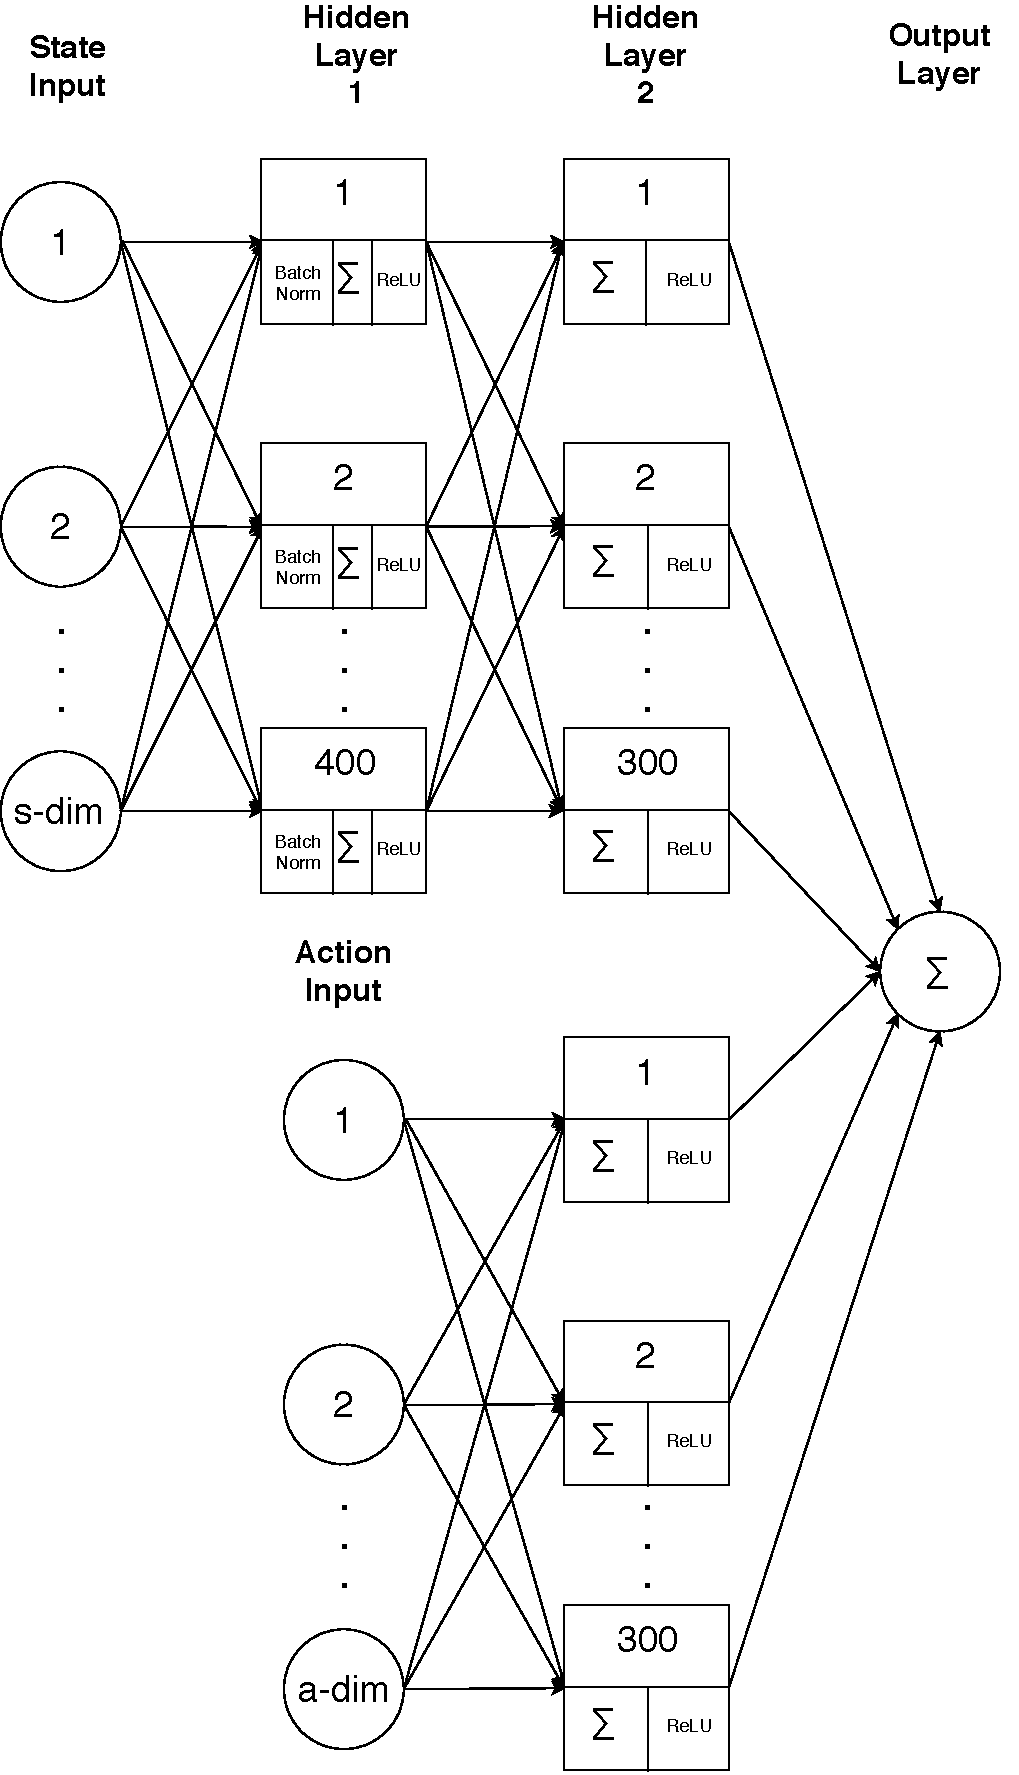
\includegraphics[width=6in, height=8.5in, keepaspectratio]{figures/critic_net.pdf}
	\caption{Critic ANN Structure}\label{fig:critic_net}
\end{figure}

\begin{python}[caption={Critic Network Class},label={list:critic_net}]
CRITIC_L1_NODES = 400
CRITIC_L2_NODES = 300

class CriticNetwork(object):
    """
    Input to the network is the state and action, output is Q(s,a).
    The action must be obtained from the output of the Actor network.

    """

    def __init__(self, sess, state_dim, action_dim, learning_rate, tau, gamma, num_actor_vars):
        self.sess = sess
        self.s_dim = state_dim
        self.a_dim = action_dim
        self.learning_rate = learning_rate
        self.tau = tau
        self.gamma = gamma

        # Create the critic network
        self.inputs, self.action, self.out = self.create_critic_network()

        self.network_params = tf.trainable_variables()[num_actor_vars:]

        # Target Network
        self.target_inputs, self.target_action, self.target_out = self.create_critic_network()

        self.target_network_params = tf.trainable_variables()[(len(self.network_params) + num_actor_vars):]

        # Op for periodically updating target network with online network
        # weights with regularization
        self.update_target_network_params = [self.target_network_params[i].assign( \
            tf.multiply(self.network_params[i], self.tau) + \
            tf.multiply(self.target_network_params[i], 1. - self.tau)) \
                for i in range(len(self.target_network_params))]

        # Network target (y_i)
        self.predicted_q_value = tf.placeholder(tf.float32, [None, 1])

        # Define loss and optimization Op
        self.loss = tflearn.mean_square(self.predicted_q_value, self.out)
        self.optimize = tf.train.AdamOptimizer(
            self.learning_rate).minimize(self.loss)

        # Get the gradient of the net w.r.t. the action.
        # For each action in the mini-batch (i.e., for each x in xs),
        # this will sum up the gradients of each critic output in the mini-batch
        # w.r.t. that action. Each output is independent of all
        # actions except for one.
        self.action_grads = tf.gradients(self.out, self.action)

        self.num_trainable_vars = len(
            self.network_params) + len(self.target_network_params)


    def create_critic_network(self):
        inputs = tflearn.input_data(shape=[None, self.s_dim], name='CriticInputs')
        action = tflearn.input_data(shape=[None, self.a_dim], name='CriticAction')
        net = tflearn.fully_connected(inputs, CRITIC_L1_NODES, name='CriticInputsNet')
        net = tflearn.layers.normalization.batch_normalization(net)
        net = tflearn.activations.relu(net)

        # Add the action tensor in the 2nd hidden layer
        # Use two temp layers to get the corresponding weights and biases
        t1 = tflearn.fully_connected(net, CRITIC_L2_NODES, name='CriticNetT1')
        t2 = tflearn.fully_connected(action, CRITIC_L2_NODES, name='CriticActionT2')

        net = tflearn.activation(
            tf.matmul(net, t1.W) + tf.matmul(action, t2.W) + t2.b, activation='relu')

        # linear layer connected to 1 output representing Q(s,a)
        # Weights are init to Uniform[-3e-3, 3e-3]
        w_init = tflearn.initializations.uniform(minval=-0.003, maxval=0.003)
        out = tflearn.fully_connected(net,1, weights_init=w_init,name='CriticNetOut')
        return inputs, action, out

    def train(self, inputs, action, predicted_q_value):
        return self.sess.run([self.out, self.optimize], feed_dict={
            self.inputs: inputs,
            self.action: action,
            self.predicted_q_value: predicted_q_value
        })

    def predict(self, inputs, action):
        return self.sess.run(self.out, feed_dict={
            self.inputs: inputs,
            self.action: action
        })

    def predict_target(self, inputs, action):
        return self.sess.run(self.target_out, feed_dict={
            self.target_inputs: inputs,
            self.target_action: action
        })

    def action_gradients(self, inputs, actions):
        return self.sess.run(self.action_grads, feed_dict={
            self.inputs: inputs,
            self.action: actions
        })

    def update_target_network(self):
        self.sess.run(self.update_target_network_params)
\end{python}

\subsubsection{Actor Network}
Listing \ref{list:actor_net} implements the actor ANN. The function \pythoninline{create_actor_network()} at line 56 defines the TensorFlow graph of the network. The actor uses an \pythoninline{s_dim}-node input layer, two fully connected hidden layers, and a  \pythoninline{a_dim}-node output layer, illustrated in Figure \ref{fig:actor_net}. The two hidden layers consist of a fully connected network layer of weights with biases, a batch normalization layer described previously, and the ReLU activation function. The two hidden layers use 400 and 300 nodes, respectively, matching Lillicrap's implementation \cite{lillicrap_2016}. Finally, the output layer is a fully connected network, tanh activation function to limit the output to $[-1,+1]$, and a multiplier to scale the output to $[-$\pythoninline{action_bound}$,+$\pythoninline{action_bound}$]$.

The \pythoninline{train()} function implements the key idea of the policy gradient method. The gradient of the output with respect to the network weights and biases are calculated and weighted the by the action gradients obtained from the critic. The weighting step effectively makes "good" actions more likely and "bad" actions less likely. The gradients are normalized by the batch size and then applied to the network weights and biased according to the Adam optimization method. 
\begin{figure}[H]   % [h] means here
	\centering 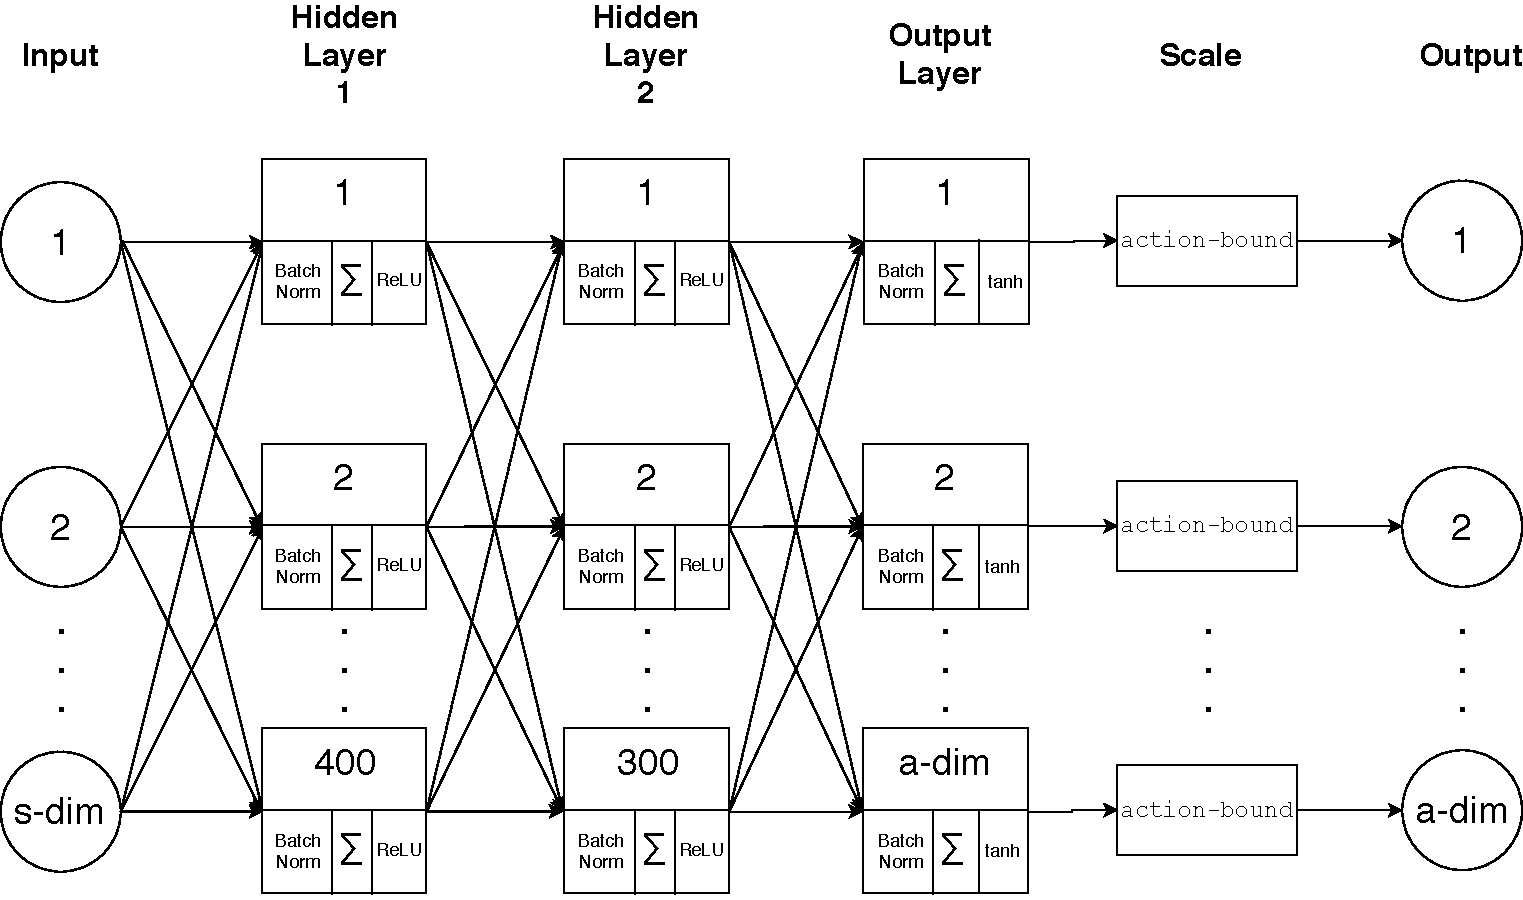
\includegraphics[width=6in, height=3.85in, keepaspectratio]{figures/actor_net.pdf}
	\caption{Actor ANN Structure}\label{fig:actor_net}
\end{figure}

\begin{python}[caption={Actor Network Class},label={list:actor_net}]
ACTOR_L1_NODES = 400
ACTOR_L2_NODES = 300

class ActorNetwork(object):
    """
    Input to the network is the state, output is the action
    under a deterministic policy.

    The output layer activation is a tanh to keep the action
    between -action_bound and action_bound
    """

    def __init__(self, sess, state_dim, action_dim, action_bound, learning_rate, tau, batch_size):
        self.sess = sess
        self.s_dim = state_dim
        self.a_dim = action_dim
        self.action_bound = action_bound
        self.learning_rate = learning_rate
        self.tau = tau
        self.batch_size = batch_size

        # Actor Network
        self.inputs, self.out, self.scaled_out = self.create_actor_network()

        self.network_params = tf.trainable_variables()

        # Target Network
        self.target_inputs, self.target_out, self.target_scaled_out = self.create_actor_network()

        self.target_network_params = tf.trainable_variables()[
            len(self.network_params):]

        # Op for periodically updating target network with online network
        # weights
        self.update_target_network_params = [self.target_network_params[i].assign( \
                tf.multiply(self.network_params[i], self.tau) + \
                tf.multiply(self.target_network_params[i], 1. - self.tau))
                for i in range(len(self.target_network_params))]

        # This gradient will be provided by the critic network
        self.action_gradient = tf.placeholder(tf.float32, [None, self.a_dim])

        # Combine the gradients here
        self.unnormalized_actor_gradients = tf.gradients(
            self.scaled_out, self.network_params, -self.action_gradient)
        self.actor_gradients = list(map(lambda x: tf.div(x, self.batch_size), 
            self.unnormalized_actor_gradients))

        # Optimization Op
        self.optimize = tf.train.AdamOptimizer(self.learning_rate).\
            apply_gradients(zip(self.actor_gradients, self.network_params))

        self.num_trainable_vars = len(
            self.network_params) + len(self.target_network_params)

    def create_actor_network(self):
        inputs = tflearn.input_data(shape=[None, self.s_dim], name='ActorInputs')
        net = tflearn.fully_connected(inputs, ACTOR_L1_NODES, name='ActorInputsNet')
        net = tflearn.layers.normalization.batch_normalization(net, name='ActorBatchNorm1Net')
        net = tflearn.activations.relu(net)
        net = tflearn.fully_connected(net, ACTOR_L2_NODES, name='ActorNetNet')
        net = tflearn.layers.normalization.batch_normalization(net, name='ActorBatchNorm2Net')
        net = tflearn.activations.relu(net)
        # Final layer weights are init to Uniform[-3e-3, 3e-3]
        w_init = tflearn.initializations.uniform(minval=-0.003, maxval=0.003)
        out = tflearn.fully_connected(
            net, self.a_dim, activation='tanh', weights_init=w_init, name='ActorOutNet')
        # Scale output to -action_bound to action_bound
        scaled_out = tf.multiply(out, self.action_bound)
        return inputs, out, scaled_out

    def train(self, inputs, a_gradient):
        self.sess.run(self.optimize, feed_dict={
            self.inputs: inputs,
            self.action_gradient: a_gradient
        })

    def predict(self, inputs):
        return self.sess.run(self.scaled_out, feed_dict={
            self.inputs: inputs
        })

    def predict_target(self, inputs):
        return self.sess.run(self.target_scaled_out, feed_dict={
            self.target_inputs: inputs
        })

    def update_target_network(self):
        self.sess.run(self.update_target_network_params)

    def get_num_trainable_vars(self):
        return self.num_trainable_vars
\end{python}

Both actor and critic classes create a regular and target network in the \pythoninline{__init__()} function. The target network is structurally identical to the regular actor/critic networks. Recall the network weights are denoted as $\theta_i$ while target network weights use $\theta^-_i$. Each class provides a function \pythoninline{update_target_network()}  that adjusts target network weights to be closer to the regular network weights by the factor $\tau=0.001$ as in Equation \ref{eq:target_update}. The \pythoninline{predict()} and \pythoninline{predict_targets()} functions return the forward pass output of the regular and target networks, respectively.
\begin{equation}
\label{eq:target_update}
\theta^-_i \gets \tau\theta_i + (1-\tau)\theta^-_i
\end{equation}

\subsection{DDPG}
Figure \ref{fig:ddpg_flow} displays the DDPG training algorithm flowchart.
\begin{figure}[H]   % [h] means here
	\centering 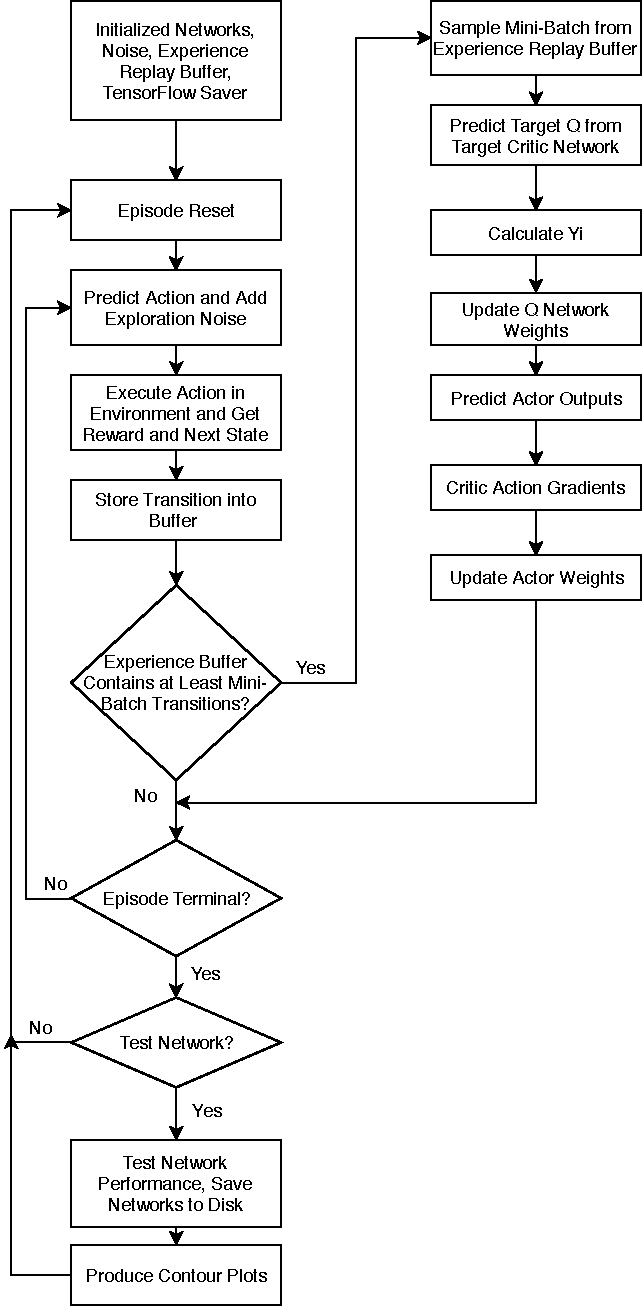
\includegraphics[width=6in, height=8.5in, keepaspectratio]{figures/ddpg_flow.pdf}
	\caption{DDPG Flowchart}\label{fig:ddpg_flow}
\end{figure}
\begin{enumerate}
\item Set training parameters such as learning rates, discount factor $\gamma$, target network update parameter $\tau$, and mini-batch size. The arguments use default values unless specified in the program arguments list.
\begin{python}[caption={Training Parameter Initialization},label={list:train_param_init},xleftmargin=\dimexpr-\csname @totalleftmargin\endcsname]
parser.add_argument('--actor-lr', help='actor network learning rate', default=0.001) 
parser.add_argument('--critic-lr', help='critic network learning rate', default=0.0001) 
parser.add_argument('--gamma', help='discount factor for critic updates', default=0.99) 
parser.add_argument('--tau', help='soft target update parameter', default=0.001) 
parser.add_argument('--buffer-size', help='max size of the replay buffer', default=1000000)
parser.add_argument('--minibatch-size', help='size of minibatch for minibatch-SGD', default=64)
\end{python}
\item Initialize the actor network, critic network, Ornstein-Uhlenbeck exploration noise, and experience replay buffer. Set the random seed to a specific value for repeatability.
\begin{python}[caption={Network, Noise, and Experience Replay Buffer Initialization},label={list:net_init},xleftmargin=\dimexpr-\csname @totalleftmargin\endcsname]
print("Instantiating actor...")
actor = ActorNetwork(sess, state_dim, action_dim, action_bound,
                     float(args['actor_lr']), float(args['tau']),
                     int(args['minibatch_size']))

print("Instantiating critic...")
critic = CriticNetwork(sess, state_dim, action_dim,
                       float(args['critic_lr']), float(args['tau']),
                       float(args['gamma']),
                       actor.get_num_trainable_vars())
actor_noise = OrnsteinUhlenbeckActionNoise(mu=np.zeros(action_dim), dt=env.dt)
replay_buffer = ReplayBuffer(int(args['buffer_size']), int(args['random_seed']))
\end{python}
\item Initialize TensorFlow variables and \pythoninline{tf.train.Saver()} for saving trained models to disk.
\begin{python}[caption={Saver Initialization},label={list:saver_init},xleftmargin=\dimexpr-\csname @totalleftmargin\endcsname]
sess.run(tf.global_variables_initializer())
saver = tf.train.Saver()
\end{python}
\item Start training loop. Each run of this loop is one episode.
	\begin{enumerate}
	\item Reset the environment randomly and get the initial state. Reset the episode reward and average max Q for each step to track actor performance.
	\begin{python}[caption={Episode Reset},label={list:ep_reset},xleftmargin=\dimexpr-\csname @totalleftmargin\endcsname]
s = env.reset()

# Track the episode reward and average max q
ep_reward = 0
ep_ave_max_q = 0
	\end{python}
	\item Start step loop. Each run of this loop is one step in the episode.
		\begin{enumerate}
		\item Predict an action (i.e. forward pass through actor network) and add Ornstein-Uhlenbeck exploration noise. Execute the action and receive a reward, next state, and if the environment is terminating. Add the transition to the experience replay buffer.
		\begin{python}[caption={Actor Predict and Step},label={list:act_pred_step},xleftmargin=\dimexpr-\csname @totalleftmargin\endcsname]
# Predict action and add exploration noise
a = actor.predict(np.reshape(s, (1, actor.s_dim))) + actor_noise()
action = a[0]

# Execute action in environment to change state
s2, r, terminal, info = env.step(action)

replay_buffer.add(np.reshape(s, (actor.s_dim,)), \
        np.reshape(action, (actor.a_dim,)), r, terminal, \
        np.reshape(s2, (actor.s_dim,)))
		\end{python}
		\item If the experience replay buffer contains at least the mini-batch number of transitions, sample a mini-batch of transitions. Use the target critic network to produce a target Q and calculate $y_i$ from the mini-batch of transitions for use in the critic loss function. Update critic and actor network weights then target critic and actor weights.
		\begin{python}[caption={Network Update},label={list:net_update},xleftmargin=\dimexpr-\csname @totalleftmargin\endcsname]
# Keep adding experience to the memory until
# there are at least minibatch size samples
if replay_buffer.size() > int(args['minibatch_size']):
	s_batch, a_batch, r_batch, t_batch, s2_batch = \
	  	replay_buffer.sample_batch(int(args['minibatch_size']))
	
	# Calculate targets
	target_q = critic.predict_target(
	  	s2_batch, actor.predict_target(s2_batch))
	
	y_i = []
	for k in range(int(args['minibatch_size'])):
	  	if t_batch[k]:
	      	y_i.append(r_batch[k])
	  	else:
	      	y_i.append(r_batch[k] + critic.gamma * target_q[k])
	
	# Update the critic given the targets
	predicted_q_value, _ = critic.train( s_batch, a_batch, \
	  	np.reshape(y_i, (int(args['minibatch_size']), 1)))
	
	ep_ave_max_q += np.amax(predicted_q_value)
	
	# Update the actor policy using the sampled gradient
	a_outs = actor.predict(s_batch)
	grads = critic.action_gradients(s_batch, a_outs)
	actor.train(s_batch, grads[0])
	
	# Update target networks
	actor.update_target_network()
	critic.update_target_network()
		\end{python}	
		\end{enumerate}
	\item Update state for the next step and increment episode reward.
	\begin{python}[caption={Step Cleanup},label={list:ep_clean},xleftmargin=\dimexpr-\csname @totalleftmargin\endcsname]
# Update state for next step
s = s2

# Increment episode reward
ep_reward += r
	\end{python}
	\item If the environment is terminated, break out of the episode. Otherwise, loop back.
	\begin{python}[caption={Episode Termination},label={list:ep_term},xleftmargin=\dimexpr-\csname @totalleftmargin\endcsname]
# End of episode
if terminal:
  	break
	\end{python}
	\item Print episode information to track progress.
	\begin{python}[caption={Print Episode Results},label={list:print_ep},xleftmargin=\dimexpr-\csname @totalleftmargin\endcsname]
print('Ep: %d | Reward: %d | Qmax: %0.4f' % \
	(i, int(ep_reward), ep_ave_max_q / float(ep_len)))
	\end{python}
	\item Periodically test the network performance (detailed in the subsection Actor Testing), record test results, save network weights to file, and produce contour plots of actor and critic outputs.
	\begin{python}[caption={Network Evaluation},label={list:net_eval},xleftmargin=\dimexpr-\csname @totalleftmargin\endcsname]
# Test the network's performance
if (i % test_period == 0):
    # Test the network and get the total reward
    print("Testing network in %d cases..." % (num_test_cases))
    test_reward, episodes = testNetworkPerformance(env, args, actor, num_test_cases)
    plotEpisodes(env.net_index, episodes, env.dt, i+1)

    # Save network session
    filepath = "./results/%s/%s_%d_%d/model.ckpt" % (sess_dir, args['env'], i+1,int(test_reward))
    save_path = saver.save(sess, filepath)

    # Contour plots of ANN output
    if (args['env'] != 'all'):
        plotANN(env.net_index, actor, i+1, 0)
        plotANN(env.net_index, critic, i+1, 1)
	\end{python}	
	\end{enumerate}
\end{enumerate}

\subsection{Actor Testing}
The training loop periodically tests the actor to evaluate performance with the \pythoninline{testNetworkPerformance()} function shown in Listing \ref{list:actor_testing}. The actor steps through a number of varied but predefined test cases. For example, the robot orientation $\theta$ ranges from $-\pi$ to $+\pi$. If using 11 test cases, the robot would begin at $\theta=[-\pi, -0.8\pi, -0.6\pi, -0.4\pi, -0.2\pi, 0, +0.2\pi, +0.4\pi, +0.6\pi, +0.8\pi, pi]$ to evaluate behavior at various states. Additionally, the action does not receive Ornstein-Uhlenbeck exploration noise. The function returns the average reward per episode as the measure of actor performance.
\begin{python}[caption={Actor Testing Function},label={list:actor_testing}]
# Tests the actor network against a number of test cases
def testNetworkPerformance(env, args, actor, num_test_cases = 10, render = False):
    test_total_reward = 0.0
    episodes = []

    # Test the network against random scenarios
    env.setWallCollision(True)
    for m in range(num_test_cases + 1):
        transitions = []
        s = env.reset(False, True, m, num_test_cases)
        ep_reward = 0.0
        for n in range(int(args['max_episode_len'])):
            if (args['render_env'] and render == True):
                env.render()

            # Choose action based on inputs
            a = actor.predict(np.reshape(s, (1, actor.s_dim)))
            action = a[0]

            # Execute action and get new state, reward
            s, r, terminal, info = env.step(action)
            ep_reward += r

            transition = (action, s, r)
            transitions.append(transition)
            if terminal:
                break
        episodes.append(transitions)
        test_total_reward += ep_reward

    env.setWallCollision(False)

    # Return the average test reward
    return (test_total_reward / (m+1), episodes)

\end{python}
%\begin{python}[caption={Caption},label={list:label}]
%
%\end{python}

\section{Results}
\subsection{Parameter Definitions}
Before discussing the results, some parameters must be defined. The Roborodentia field is 2438.4 mm long in the x direction and 1219.2 mm wide in the y direction as shown in Figure \ref{fig:field_defs} \cite{roborodentia}. Viewed from above, the coordinate (0,0) is the bottom-left corner while (2438.4, 1219.2) is the top-right corner. The robot position, ($x$, $y$, $\theta$), is represented as a vector in the field plane where the base of the vector is at the robot center. Note that the vector orientation deviates from standard notation; 0 radians is in line with the positive y-axis and $+\pi/2$ radians is in line with the negative x-axis. The x velocity and acceleration of the robot refer to motion parallel to the field x-axis. Three control inputs $u_x$, $u_y$, and $u_\theta$ correspond proportionally to force applied to the robot and range between -2 to +2. For absolute clarity, positive $u_x$ moves the robot in the direction of the positive x-axis, positive $u_y$ pushes towards the positive y-axis, and positive $u_\theta$ torques the robot in the positive $\theta$ direction. Robot velocities are defined similarly using ($\dot{x}$, $\dot{y}$, $\dot{\theta}$). Units of position, orientation, linear velocity, and rotational velocity are mm, mm/s, radians, and radians/s, respectively.
\begin{figure}[H]
	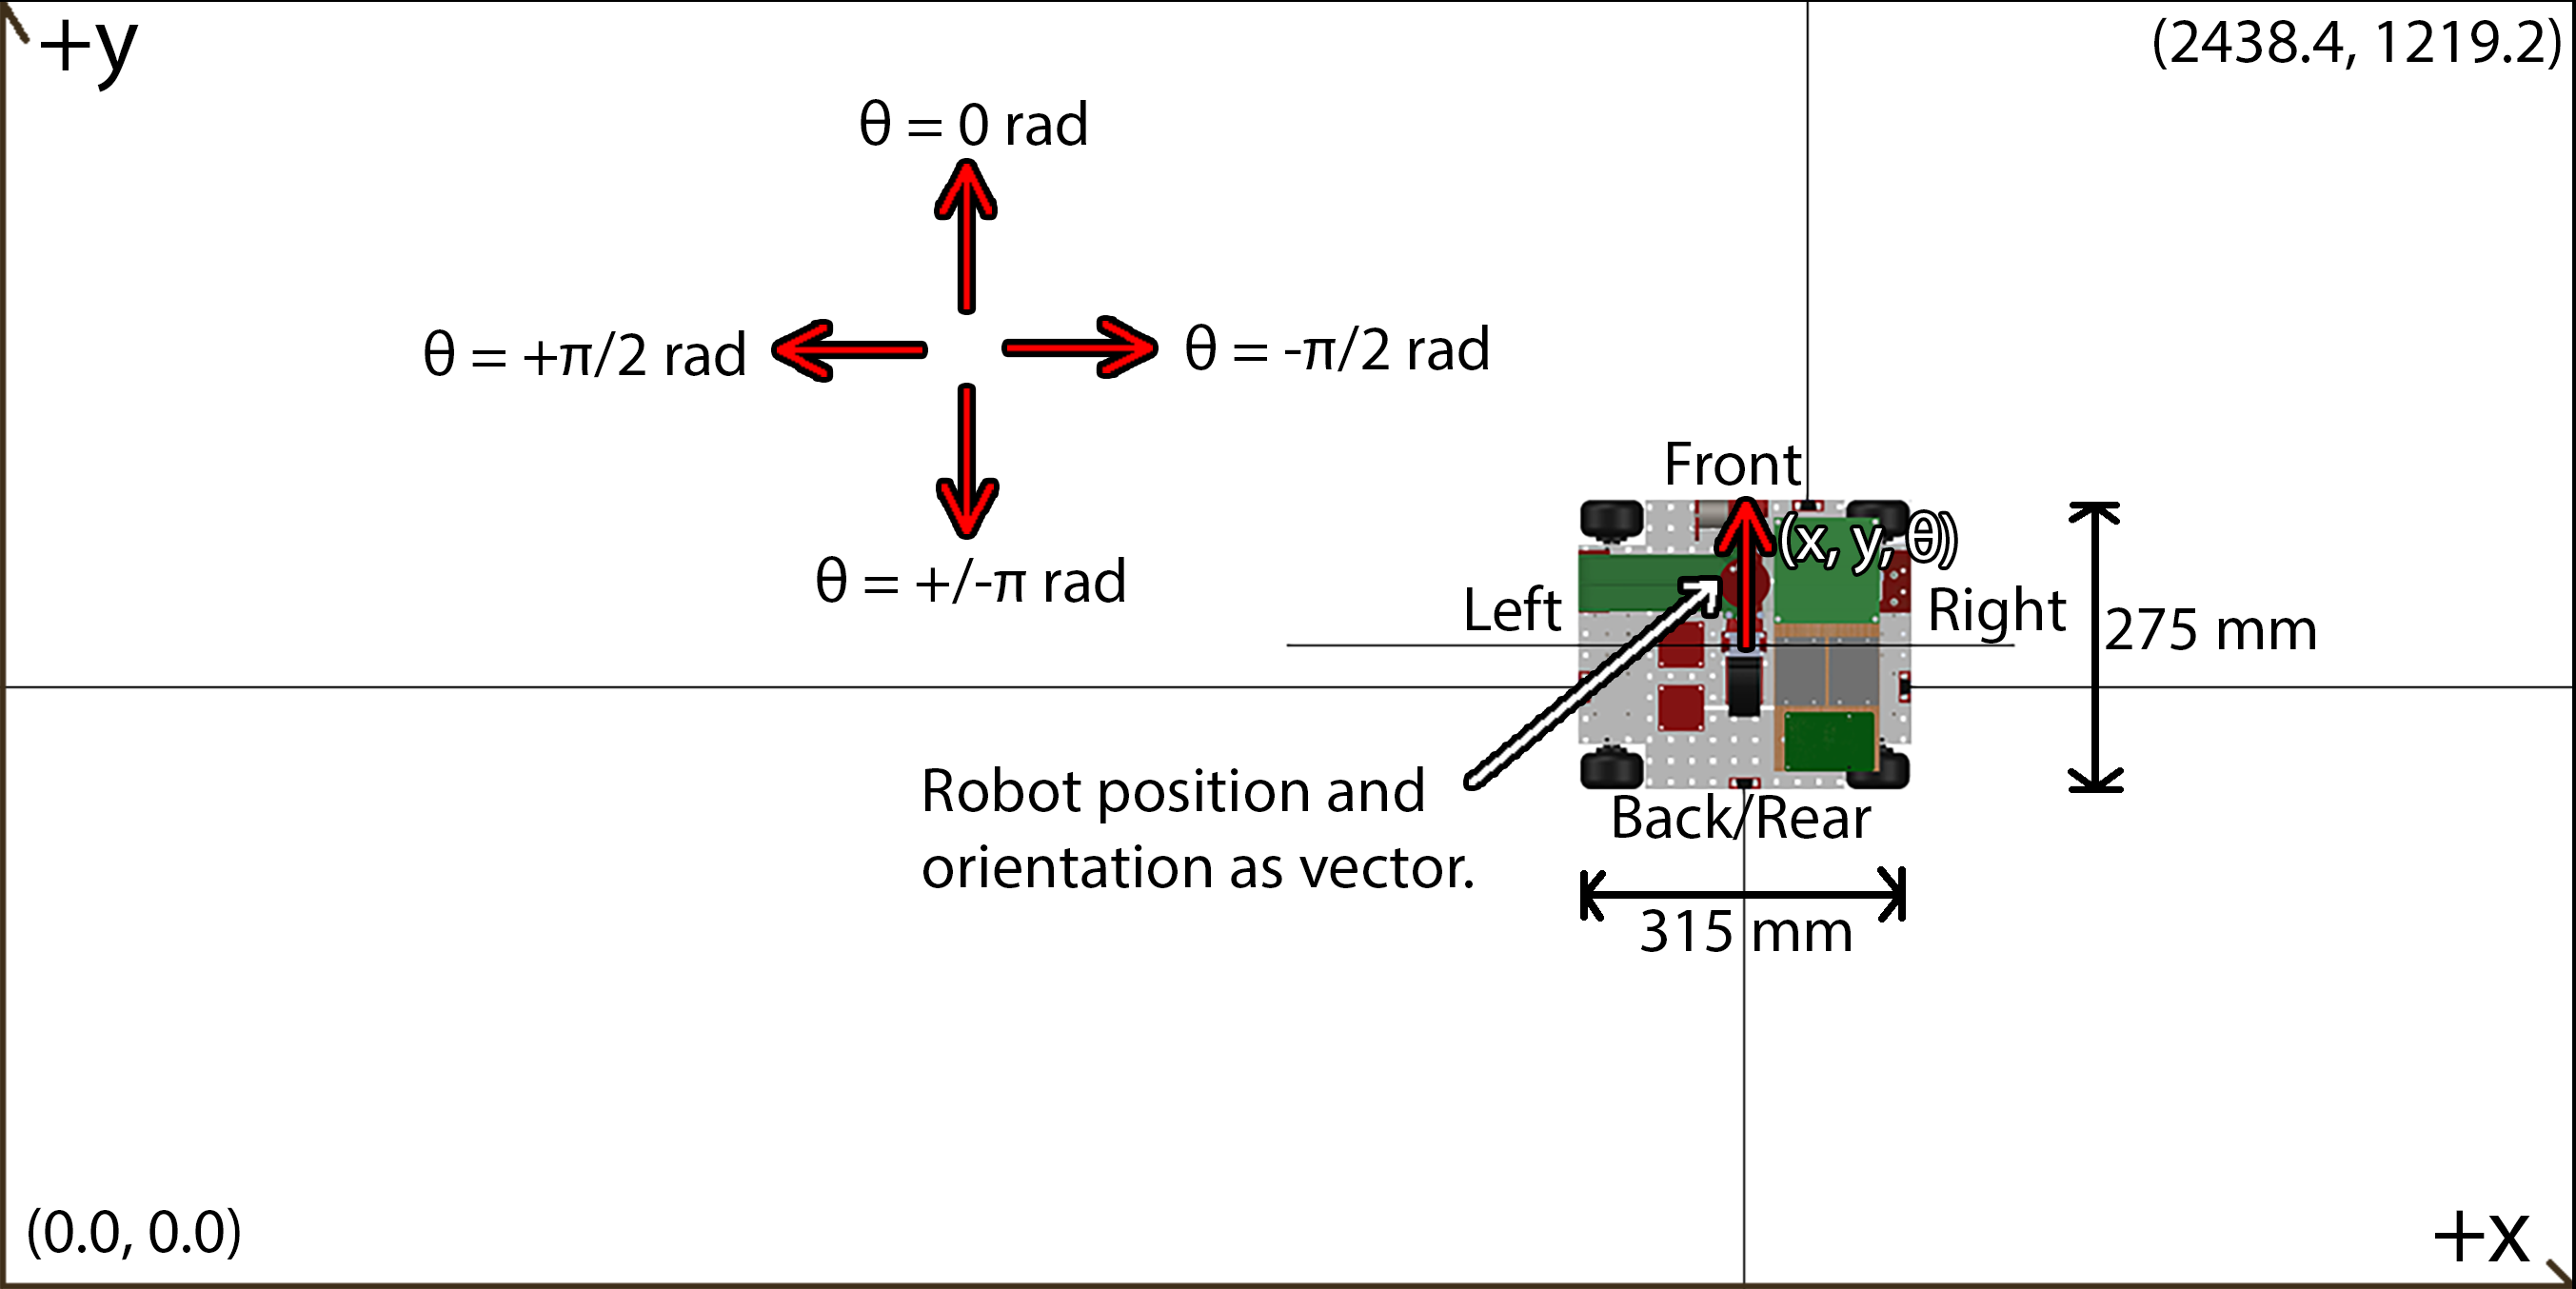
\includegraphics[width=6in, height=3.85in, keepaspectratio]{figures/field_defs.png}
	\caption{Roborodentia Field Definitions} \label{fig:field_defs}
\end{figure}

\subsection{Three Actors Variant}
Since the robot's mecanum wheels permit omni-directional movement, position control can be viewed as three separate control loops. Therefore, early experiments used three individually-trained, single-action actors to provide orthogonal controls $u_x$, $u_y$, and $u_\theta$. The three controls are converted to individual motor voltages, $v_0$, $v_1$, $v_2$, and $v_3$, by calculating the translation vector magnitude $V_d = \sqrt{u_x^2 + u_y^2}/2$ and angle $\theta_d = \text{atan2}(u_y / u_x)$ and using Equations \ref{eq:mecanum_v0} through \ref{eq:mecanum_v3} \cite{li_2018}\cite{rahman_2014}. The three actors will be referred to as the "x translation", "y translation", and "angle" networks. Each episode lasts 10 seconds with 0.05 second steps for a total of 200 steps per episode. The each network's training uses a simulation of the robot and the environment detailed in the Software chapter.
\begin{align}
v_0 &= V_d \text{sin}(\theta_d + \pi/4) - u_\theta  \label{eq:mecanum_v0}\\
v_1 &= V_d \text{cos}(\theta_d + \pi/4) + u_\theta  \label{eq:mecanum_v1}\\
v_2 &= V_d \text{sin}(\theta_d + \pi/4) + u_\theta  \label{eq:mecanum_v2}\\
v_3 &= V_d \text{cos}(\theta_d + \pi/4) - u_\theta  \label{eq:mecanum_v3}
\end{align}

\subsubsection{X Translation Network}
The x translation network takes in the robot's x error, the difference between the desired and actual x positions, and velocity and outputs $u_x$. Since the Y translation network accomplishes the exact same task in the same way but in the y direction, only the X translation network will be discussed. The reward is calculated as shown in Equation \ref{eq:x_reward}. The actor receives a higher reward for keeping the robot near the desired set point, minimizing the velocity, and minimizing the effort (i.e. low $u_x$ values).
\begin{equation}
r = -0.00001(x-x_{desired})^2-0.0000005\dot{x}^2-0.001u_x^2
\label{eq:x_reward}
\end{equation}

As described above in Actor Testing, the networks are periodically tested to observe their change in performance with more training. Figures \ref{fig:x_r} and \ref{fig:x_rzoom} show the average testing episode reward from the \pythoninline{testNetworkPerformance()} function with 41 test cases versus number of episodes trained. Figure \ref{fig:x_q} shows the average max Q versus number of episodes trained. The average max Q is calculated as the average maximum Q within each mini-batch of predicted Q's. The actor quickly learns and achieves an average test episode reward of -59 after 81 episodes. After 200 episodes, the average reward begins to decrease, indicating the possibility of over-training. However, the average max Q continues to increase.
\begin{figure}[H]
	\centering
	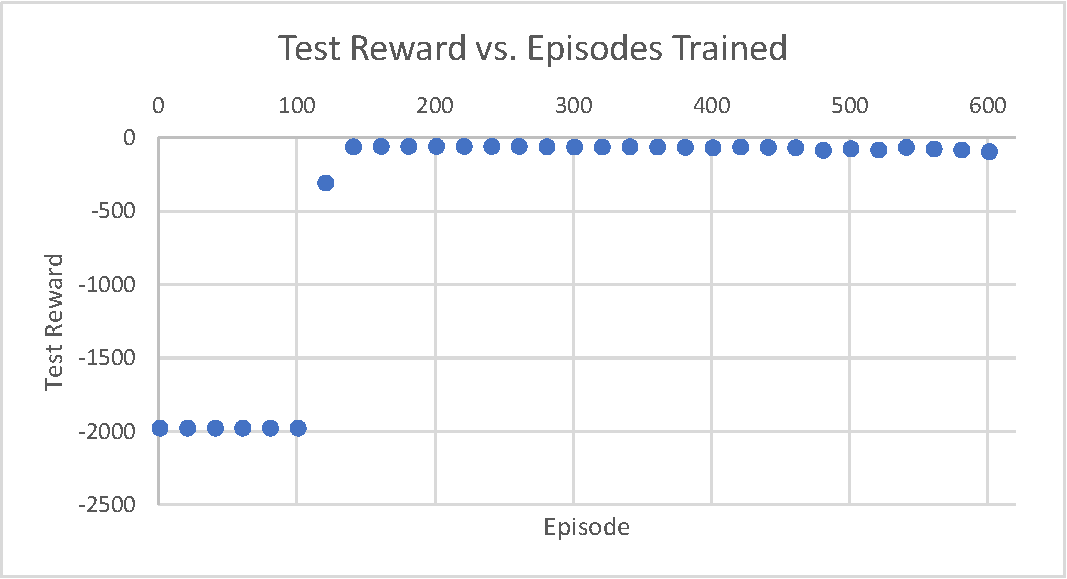
\includegraphics[width=6in, height=3.85in, keepaspectratio]{figures/train_figs/x_r.pdf}
	\caption{X Translation Test Reward} \label{fig:x_r}
\end{figure}
\begin{figure}[H]
	\centering
	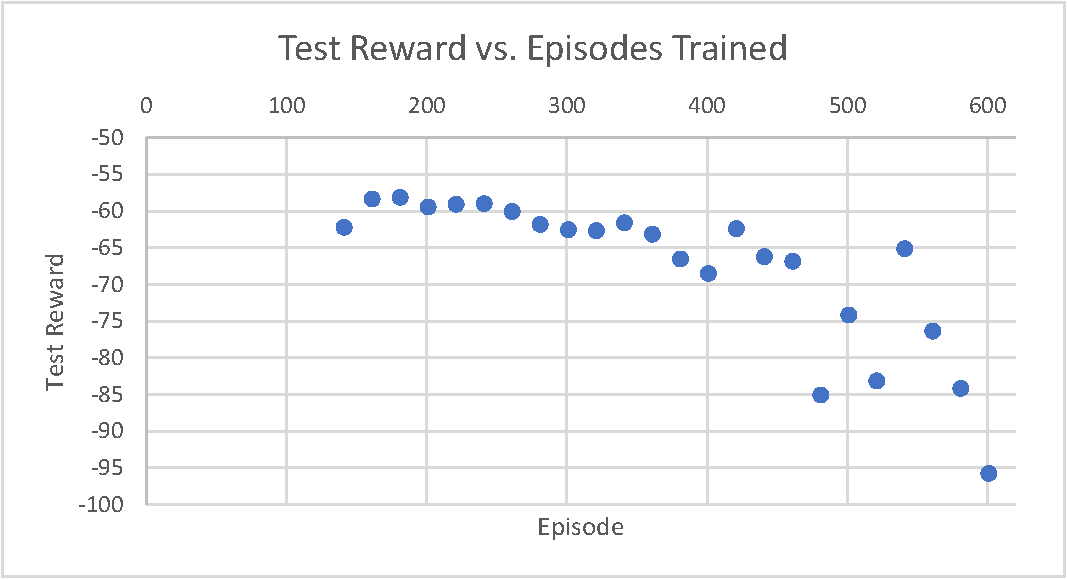
\includegraphics[width=6in, height=3.85in, keepaspectratio]{figures/train_figs/x_rzoom.pdf}
	\caption{X Translation Test Reward Zoomed} \label{fig:x_rzoom}
\end{figure}
\begin{figure}[H]
	\centering
	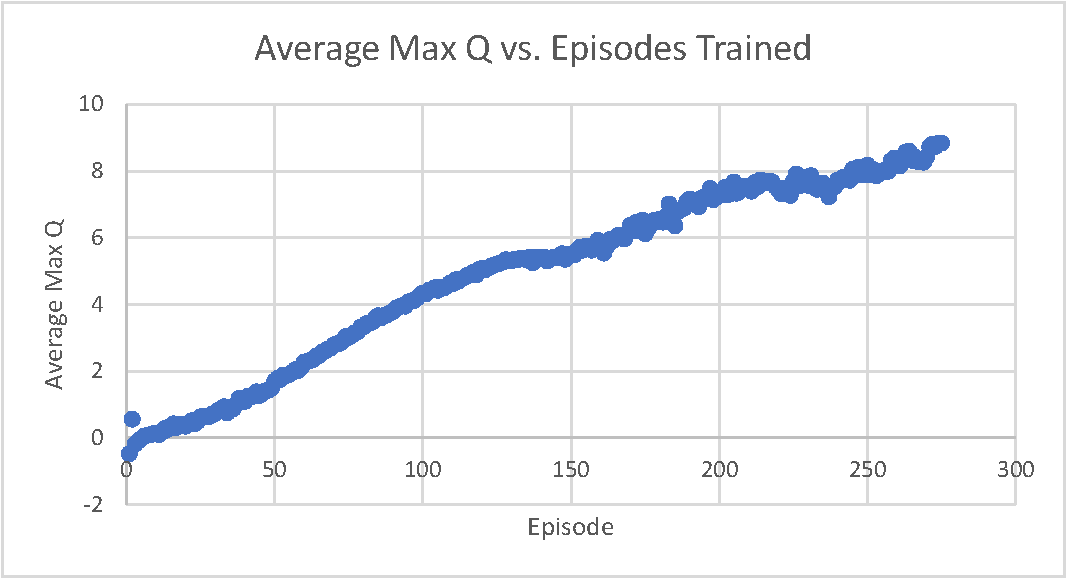
\includegraphics[width=6in, height=3.85in, keepaspectratio]{figures/train_figs/x_q.pdf}
	\caption{X Translation Network Average Max Q} \label{fig:x_q}
\end{figure}

Figure \ref{fig:x_perf} shows the actor's action, error from the set point, and reward versus time for nine different initial conditions. Appendix \ref{appendix:x_perf} provides additional plots for different numbers of episodes trained. Regardless of the starting distance from the set point, the actor appears to drive the robot at maximum speed to reach the set point as quickly as possible since the distance affects the reward most drastically. After reaching the desired x location, the action oscillates to maintain the position.
\begin{figure}[H]
	\centering
	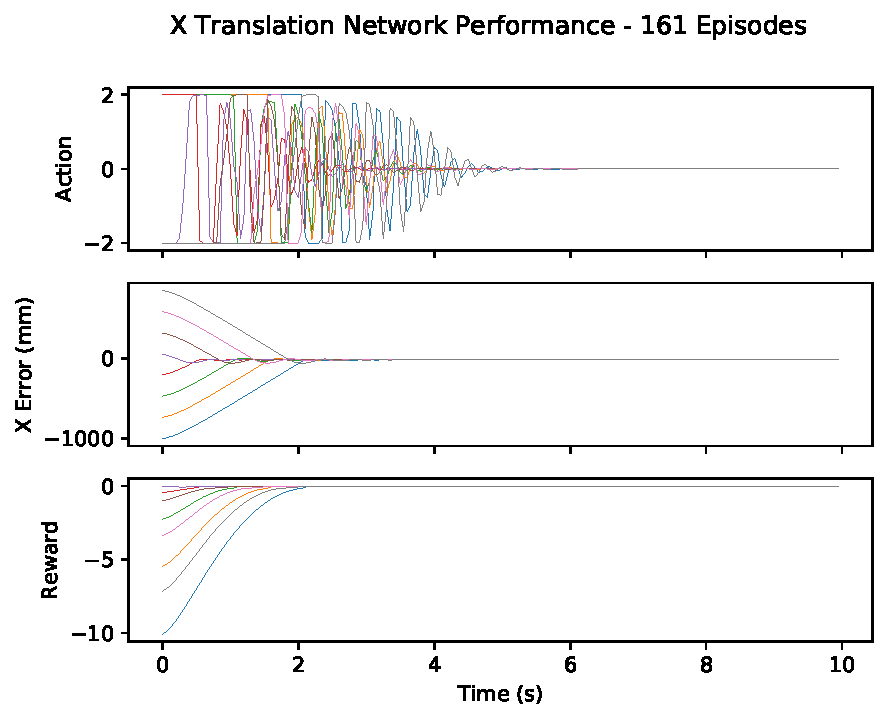
\includegraphics[width=6in, height=3.85in, keepaspectratio]{figures/train_figs/transx_transitions/1_161.pdf}
	\caption{X Translation Network Performance -- 161 Episodes}\label{fig:x_perf}
\end{figure}

Figure \ref{fig:x_actor_contour} displays a series of contour plots of the actor outputs as functions of the two inputs over different numbers of episodes trained. The actor contour plots reveal the actor output to be highly polarized with only a sliver of low-valued $u_x$, leading to the oscillatory action seen in Figure \ref{fig:x_perf}. It is highly likely that actor is incapable of sufficiently reducing the velocity such that the momentum of the robot does not carry it across the sliver and oscillating. Throughout training, the critical point at zero distance error and zero velocity yields $u_x=0$ while two "arms" of $u_x=0$ extend outward at varying angles.
\begin{figure}[H]
	\begin{tabular}{cc}
		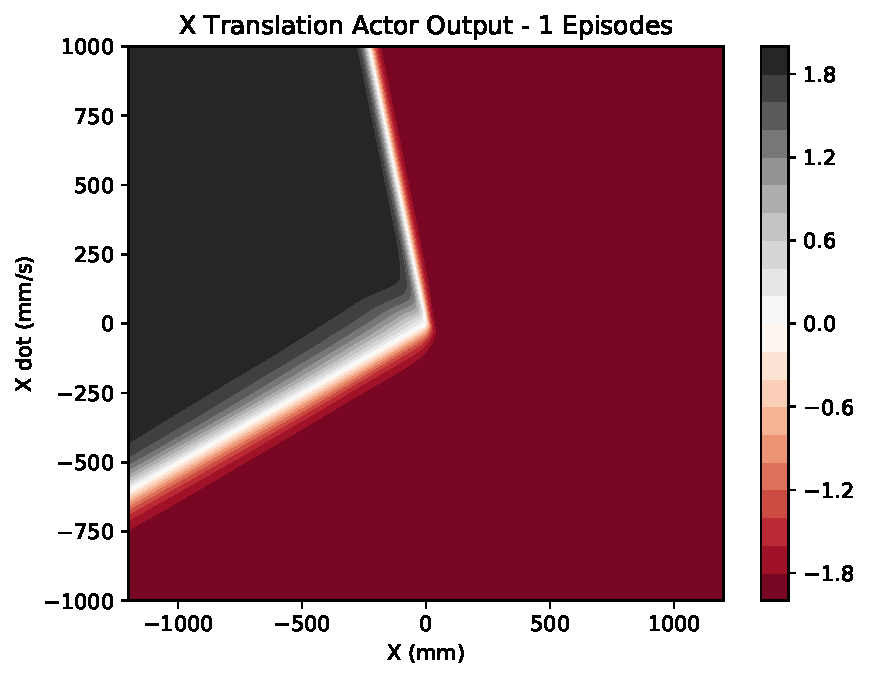
\includegraphics[width=65mm]{figures/train_figs/transx_actor/Actor1_1.pdf} &  
		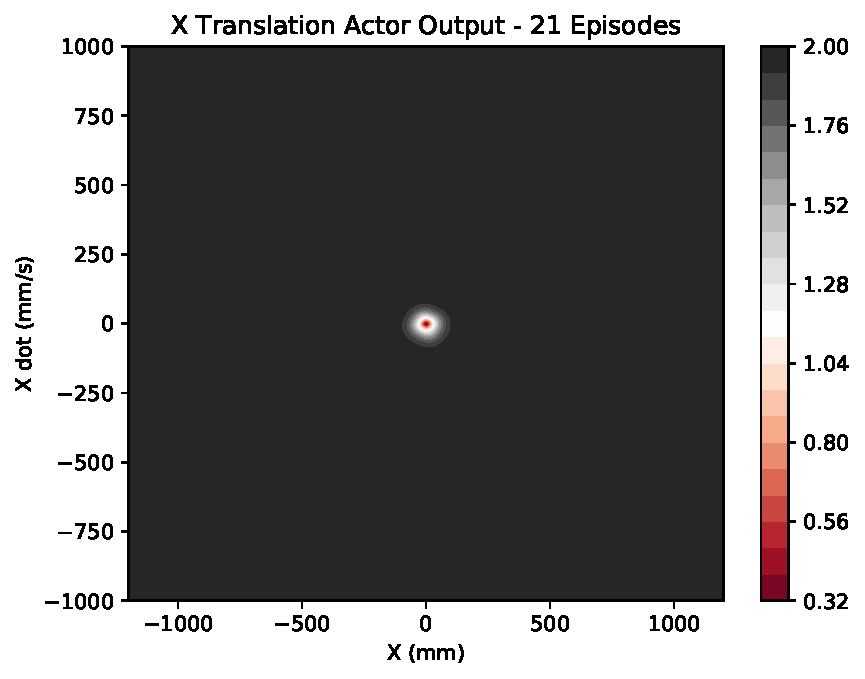
\includegraphics[width=65mm]{figures/train_figs/transx_actor/Actor1_21.pdf} \\
		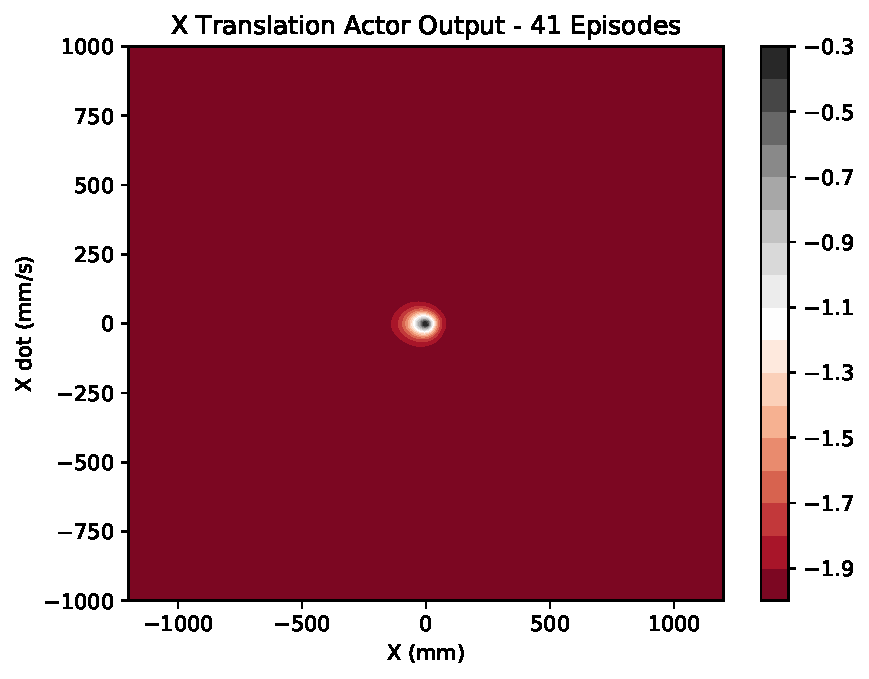
\includegraphics[width=65mm]{figures/train_figs/transx_actor/Actor1_41.pdf} &   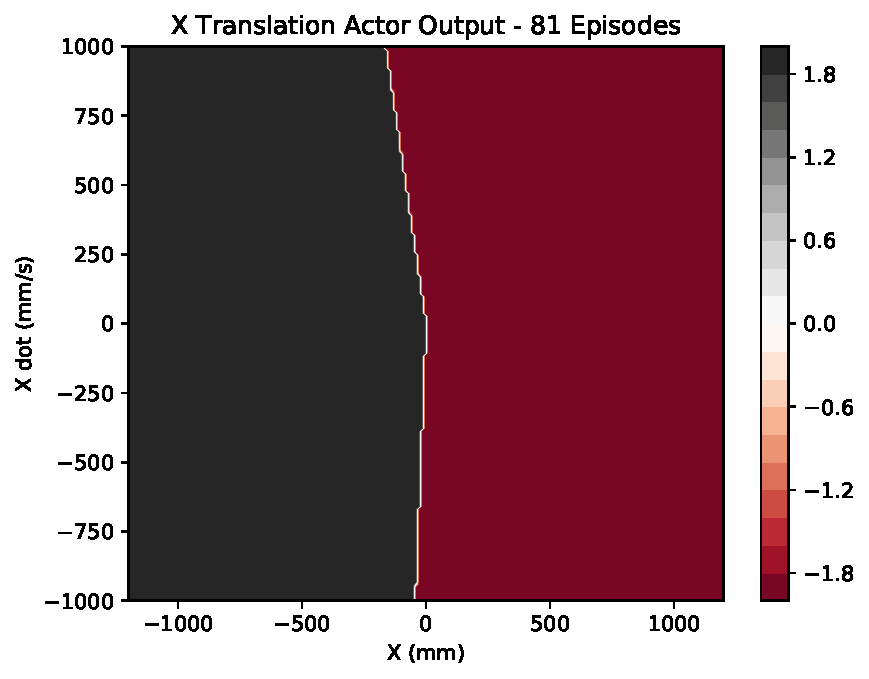
\includegraphics[width=65mm]{figures/train_figs/transx_actor/Actor1_81.pdf} \\
		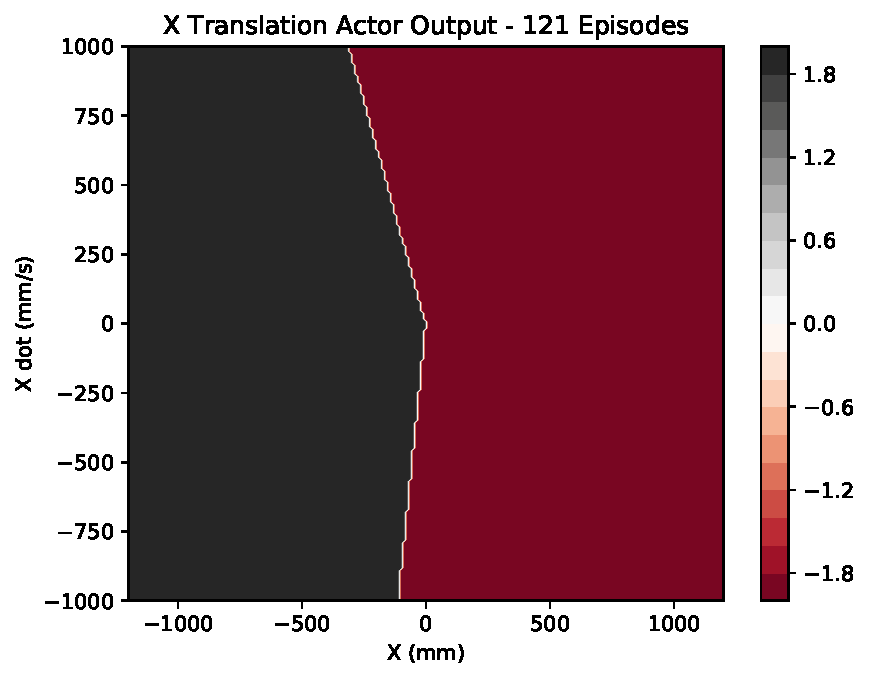
\includegraphics[width=65mm]{figures/train_figs/transx_actor/Actor1_121.pdf} &   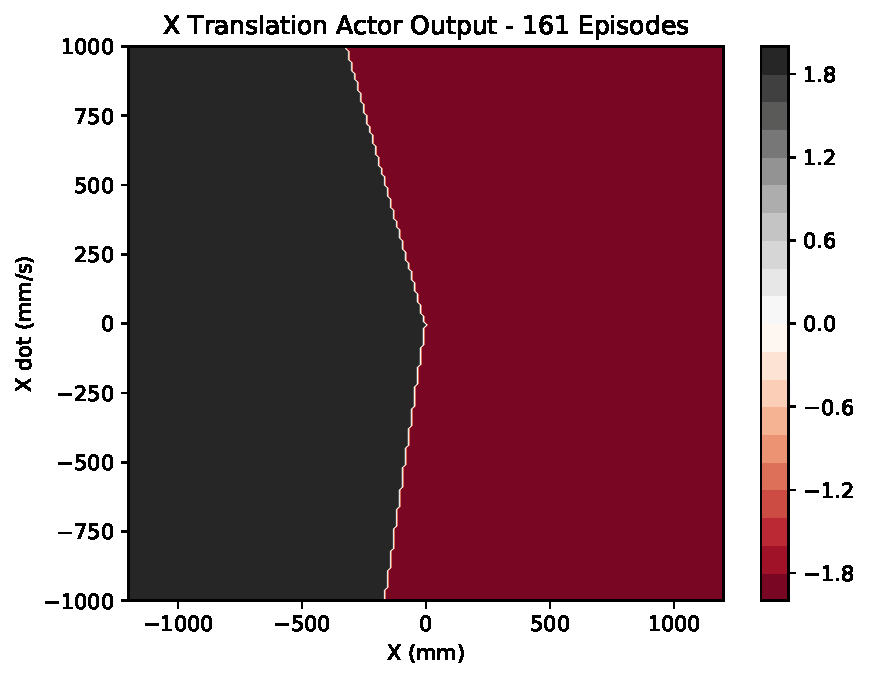
\includegraphics[width=65mm]{figures/train_figs/transx_actor/Actor1_161.pdf} \\
		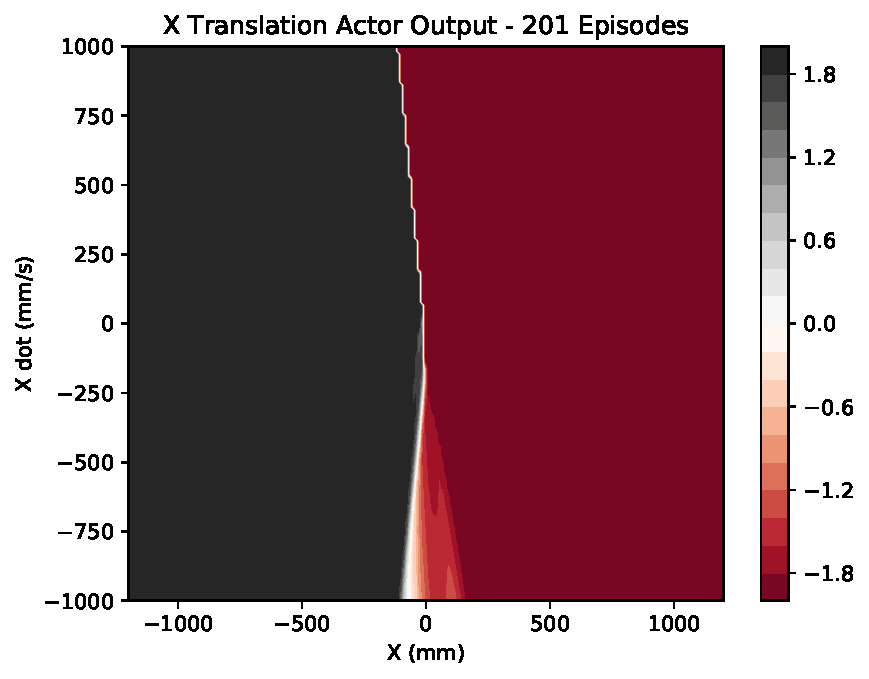
\includegraphics[width=65mm]{figures/train_figs/transx_actor/Actor1_201.pdf} &   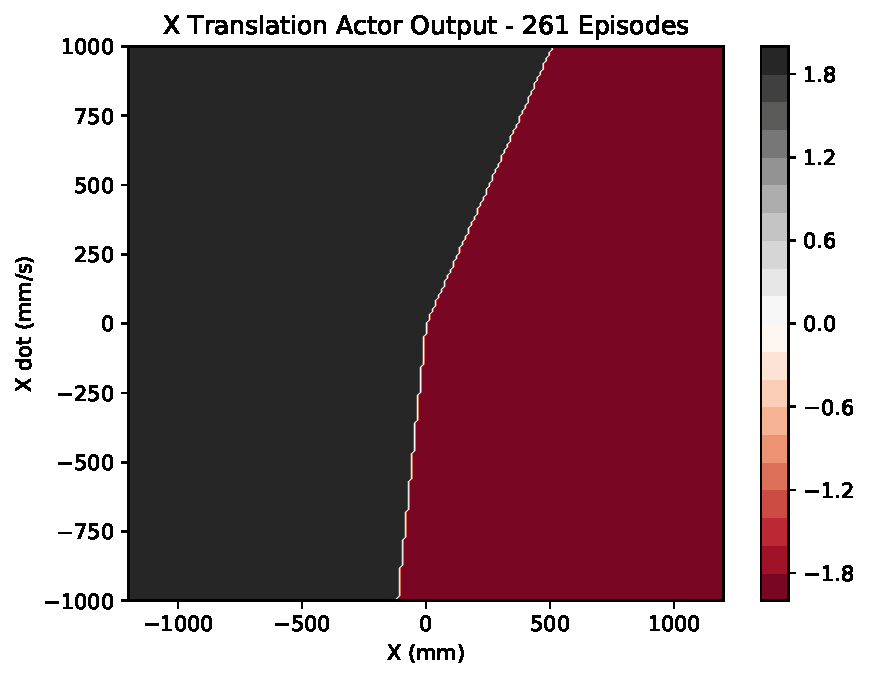
\includegraphics[width=65mm]{figures/train_figs/transx_actor/Actor1_261.pdf} \\
	\end{tabular}
	\caption{X Translation Actor Output Progression}\label{fig:x_actor_contour}
\end{figure}
\begin{figure}[H]
	\begin{tabular}{cc}
		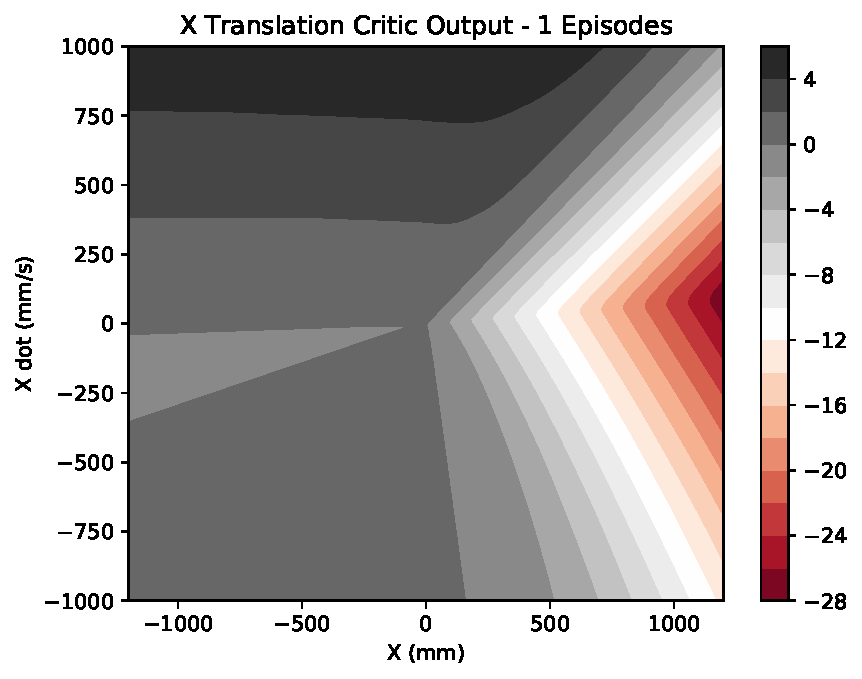
\includegraphics[width=65mm]{figures/train_figs/transx_critic/Critic1_1.pdf} &  
		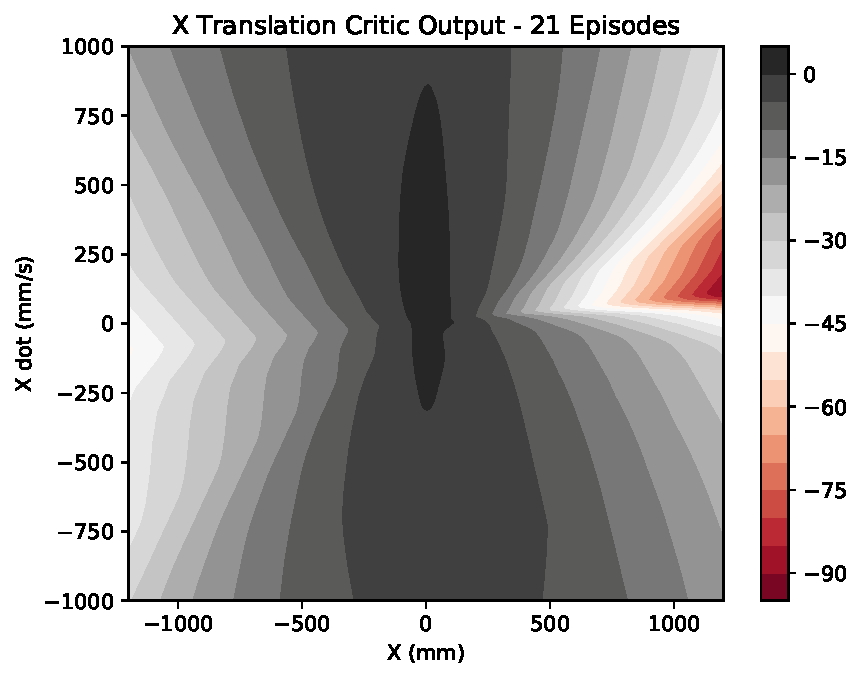
\includegraphics[width=65mm]{figures/train_figs/transx_critic/Critic1_21.pdf} \\
		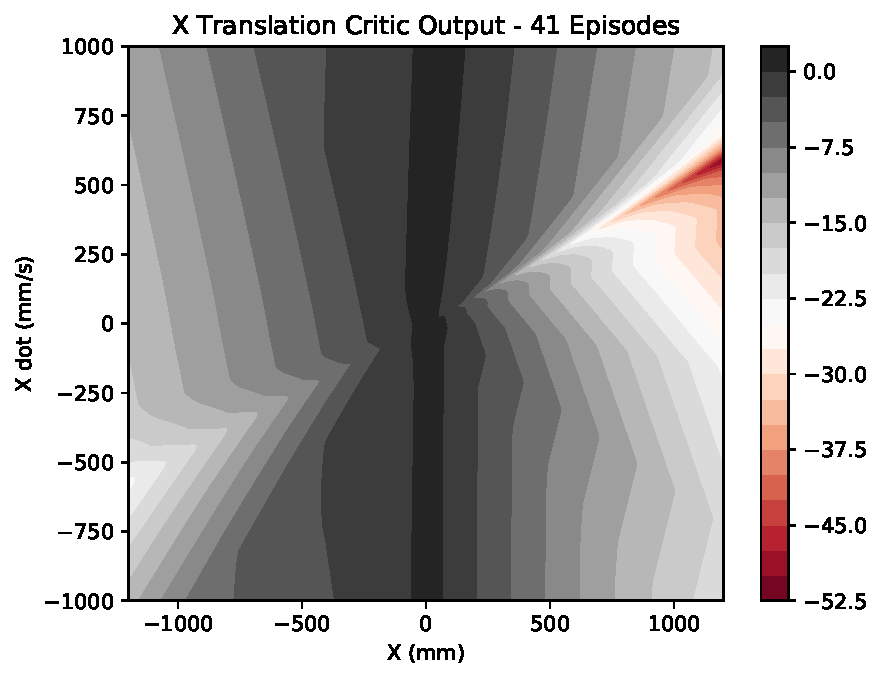
\includegraphics[width=65mm]{figures/train_figs/transx_critic/Critic1_41.pdf} &   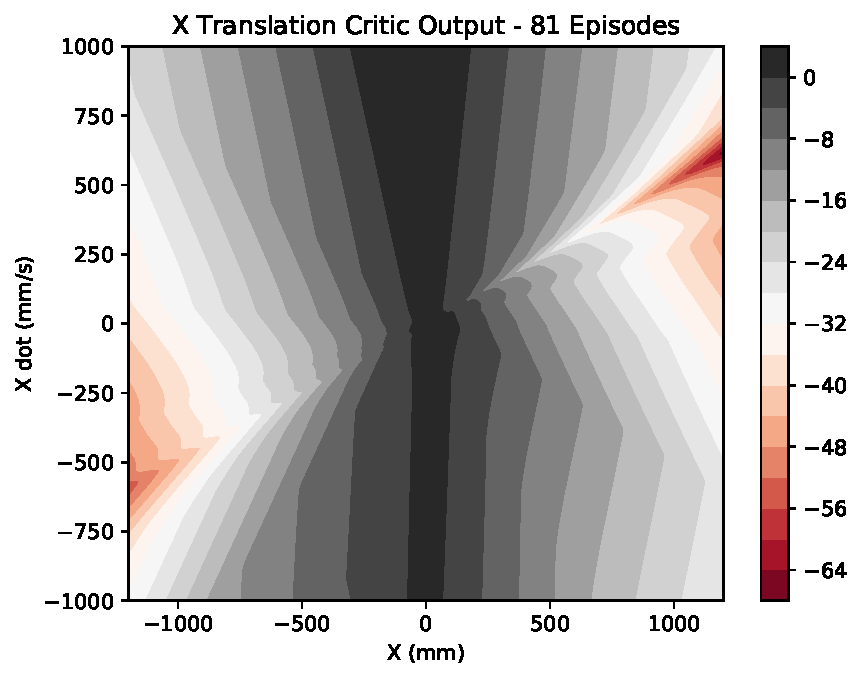
\includegraphics[width=65mm]{figures/train_figs/transx_critic/Critic1_81.pdf} \\
		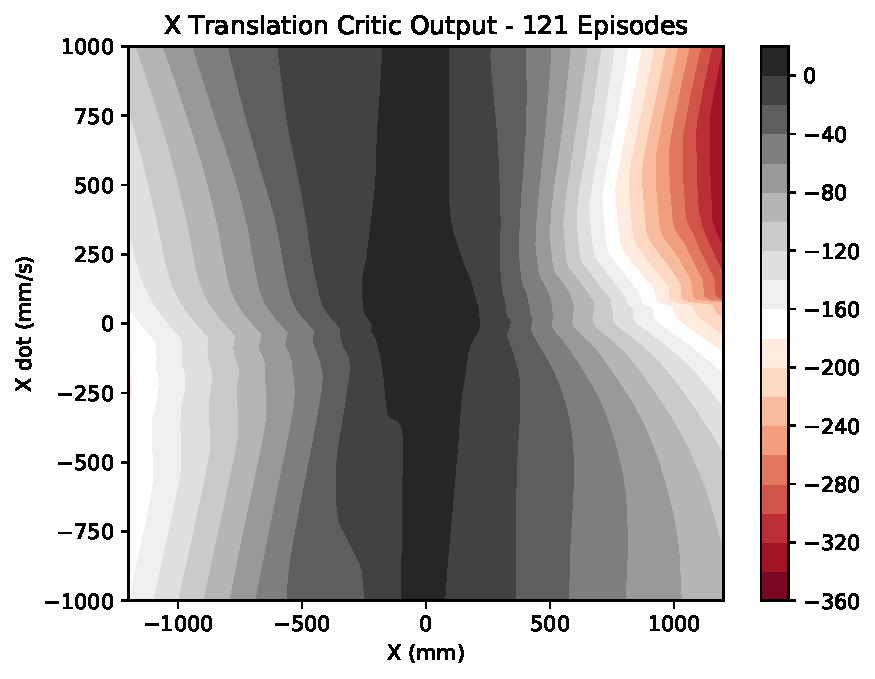
\includegraphics[width=65mm]{figures/train_figs/transx_critic/Critic1_121.pdf} &   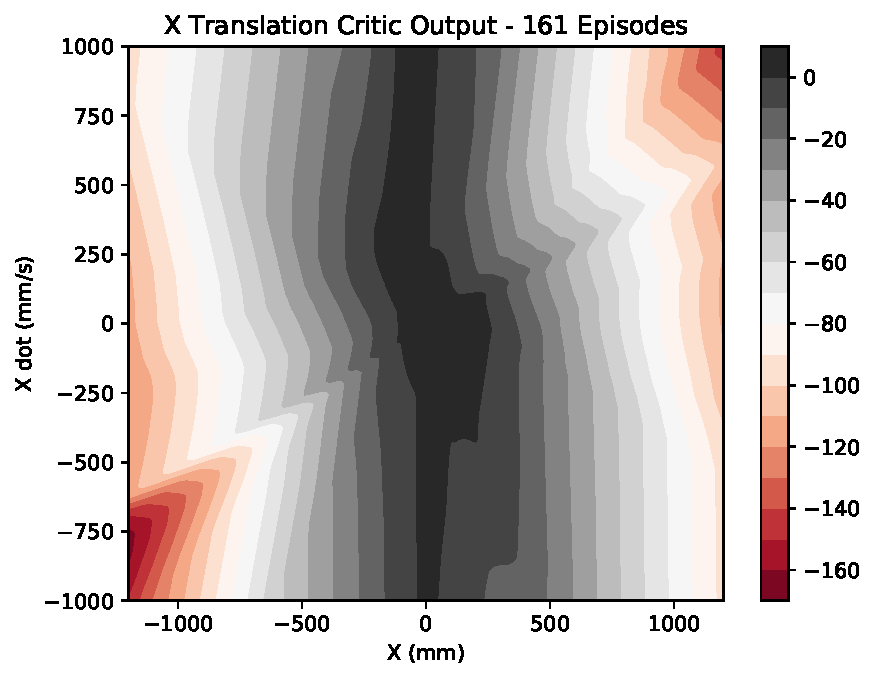
\includegraphics[width=65mm]{figures/train_figs/transx_critic/Critic1_161.pdf} \\
		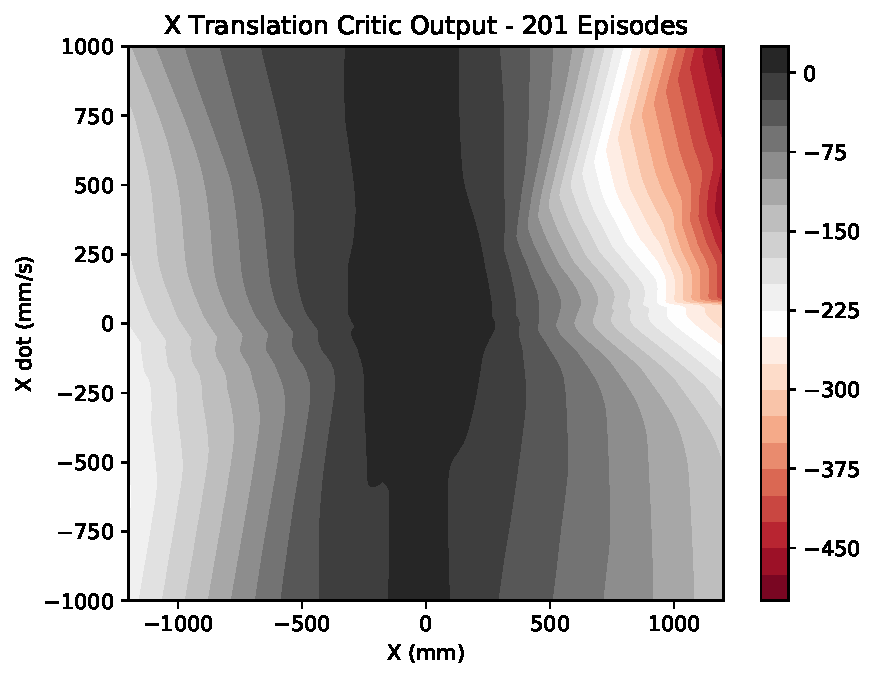
\includegraphics[width=65mm]{figures/train_figs/transx_critic/Critic1_201.pdf} &   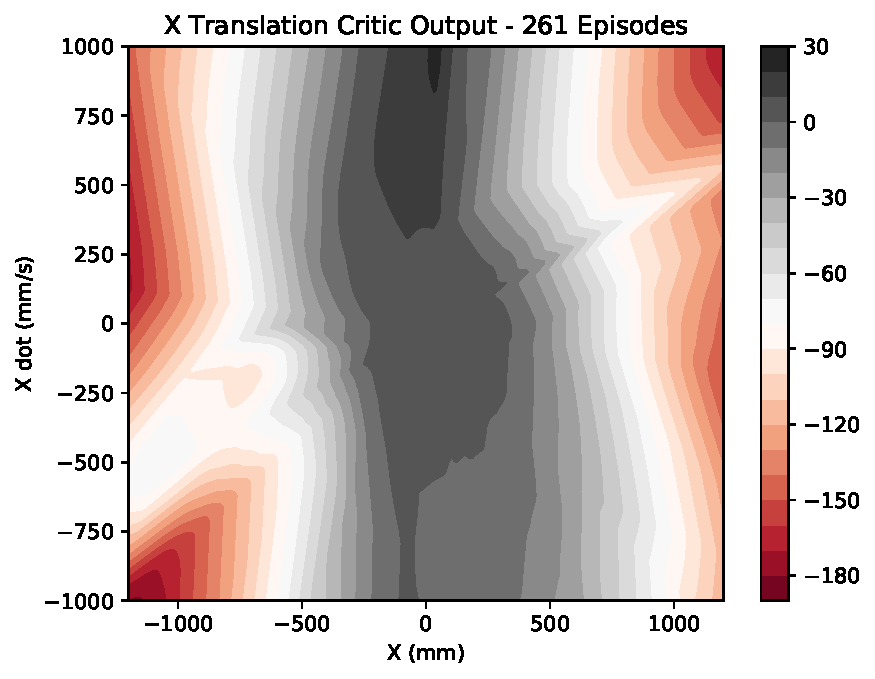
\includegraphics[width=65mm]{figures/train_figs/transx_critic/Critic1_261.pdf} \\
	\end{tabular}
	\caption{X Translation Critic Output Progression}\label{fig:x_critic_contour}
\end{figure}
Figure \ref{fig:x_critic_contour} shows a similar series of plots as Figure \ref{fig:x_actor_contour} except for the critic output rather than the actor's. Since Q is a function of both the state and action, the values shown represent the highest Q-value for any action across all states.

\subsubsection{Angle Translation Network}
The angle network takes in the robot's angle error as $\text{cos}(\theta-\theta_{desired})$ and $\text{sin}(\theta-\theta_{desired})$ as well as the rotational velocity $\dot{\theta}$ and outputs $u_\theta$. The reward is calculated as shown in Equation \ref{eq:angle_reward} where the $\text{norm}()$ function normalizes the angle to between $-\pi$ and $+\pi$.
\begin{equation}
r = -1.0(\text{norm}(\theta)-\text{norm}(\theta_{desired}))^2-0.1\dot{\theta}^2-0.001u_\theta^2
\label{eq:angle_reward}
\end{equation}

\begin{figure}[H]
	\centering
	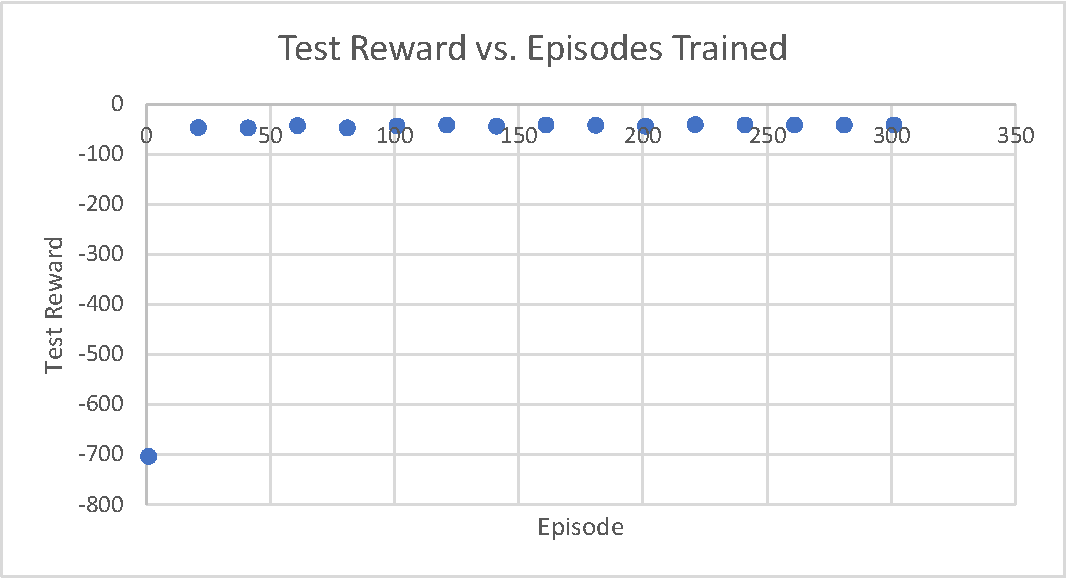
\includegraphics[width=6in, height=3.85in, keepaspectratio]{figures/train_figs/angle_r.pdf}
	\caption{Angle Test Reward} \label{fig:angle_r}
\end{figure}
\begin{figure}[H]
	\centering
	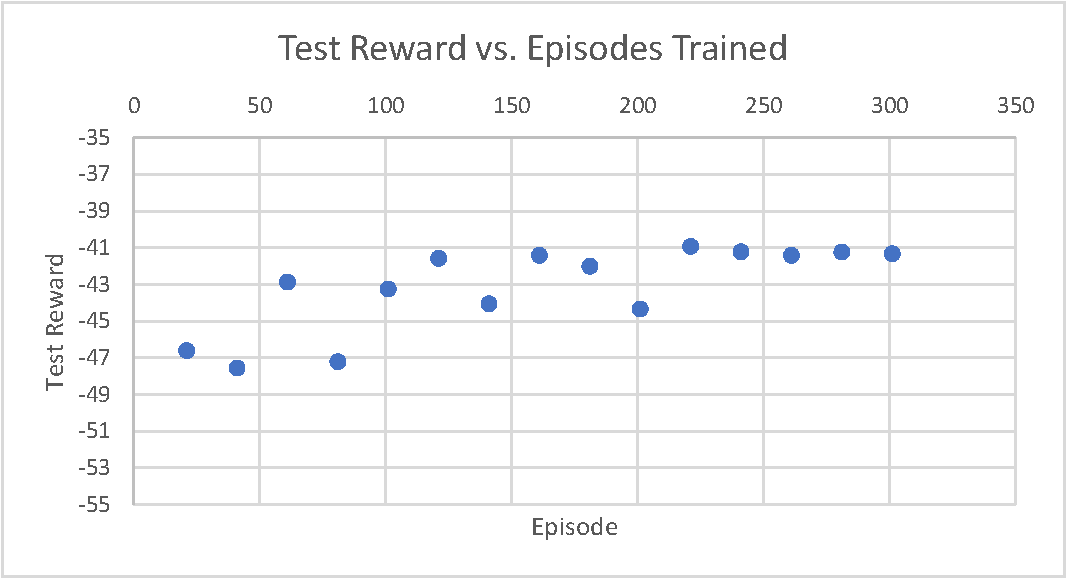
\includegraphics[width=6in, height=3.85in, keepaspectratio]{figures/train_figs/angle_rzoom.pdf}
	\caption{Angle Test Reward Zoomed} \label{fig:angle_rzoom}
\end{figure}
\begin{figure}[H]
	\centering
	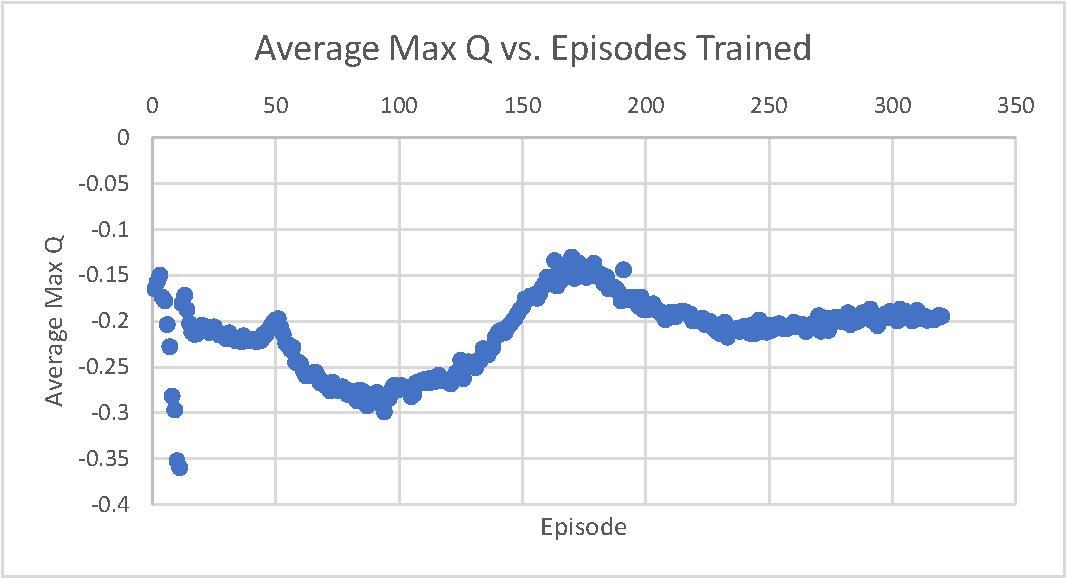
\includegraphics[width=6in, height=3.85in, keepaspectratio]{figures/train_figs/angle_q.pdf}
	\caption{Angle Network Average Max Q} \label{fig:angle_q}
\end{figure}

Appendix \ref{appendix:angle_perf} provides additional plots for different numbers of episodes trained. 
\begin{figure}[H]
	\centering
	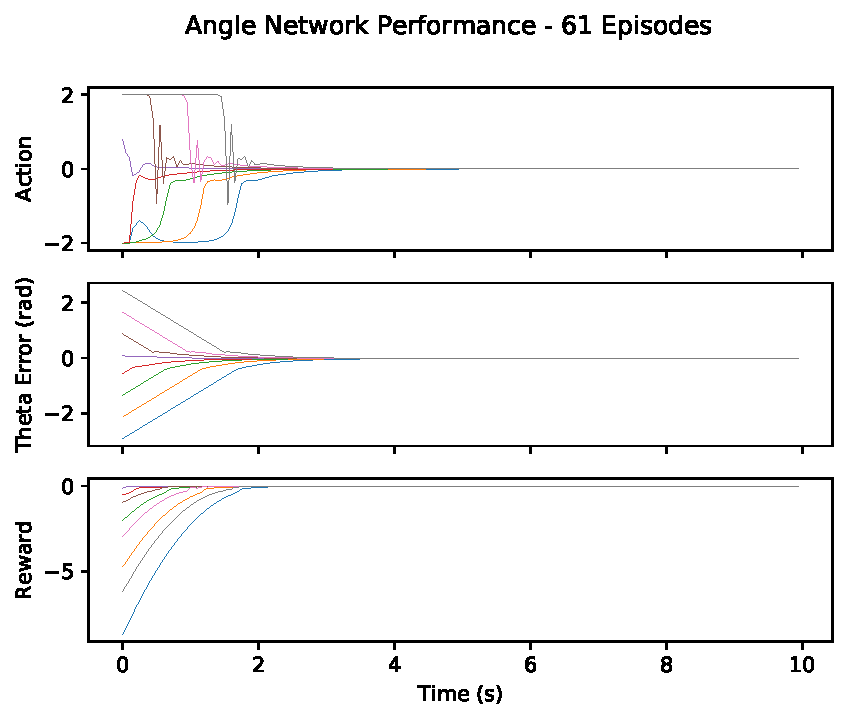
\includegraphics[width=6in, height=3.85in, keepaspectratio]{figures/train_figs/angle_transitions/0_61.pdf}
	\caption{Angle Network Performance -- 81 Episodes}\label{fig:angle_perf}
\end{figure}

\begin{figure}[H]
	\begin{tabular}{cc}
		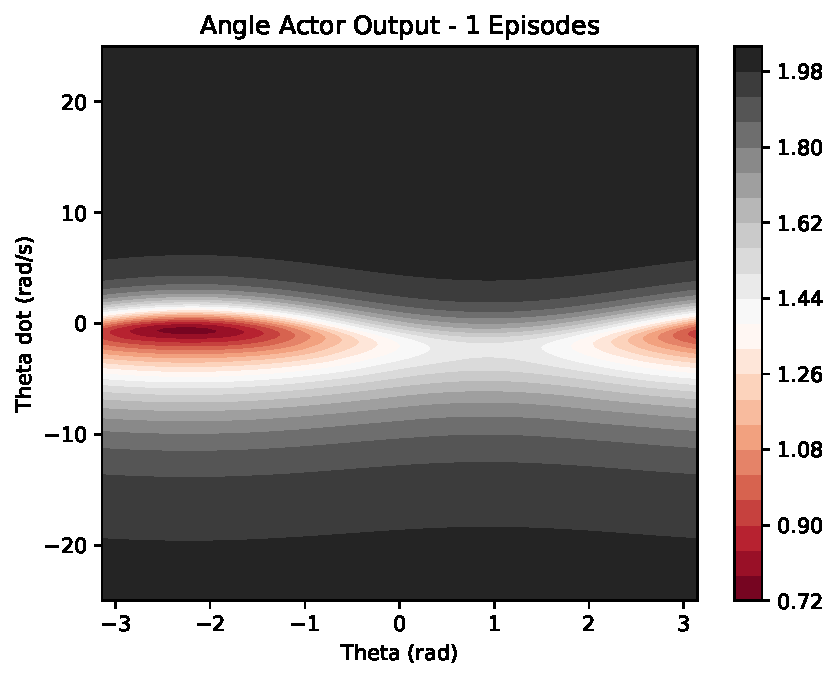
\includegraphics[width=65mm]{figures/train_figs/angle_actor/Actor0_1.pdf} &  
		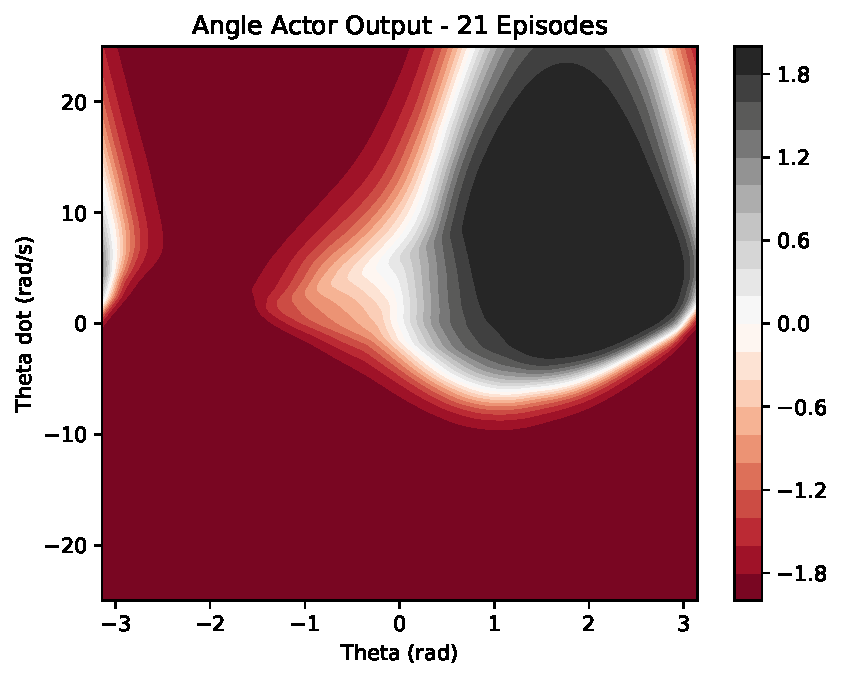
\includegraphics[width=65mm]{figures/train_figs/angle_actor/Actor0_21.pdf} \\
		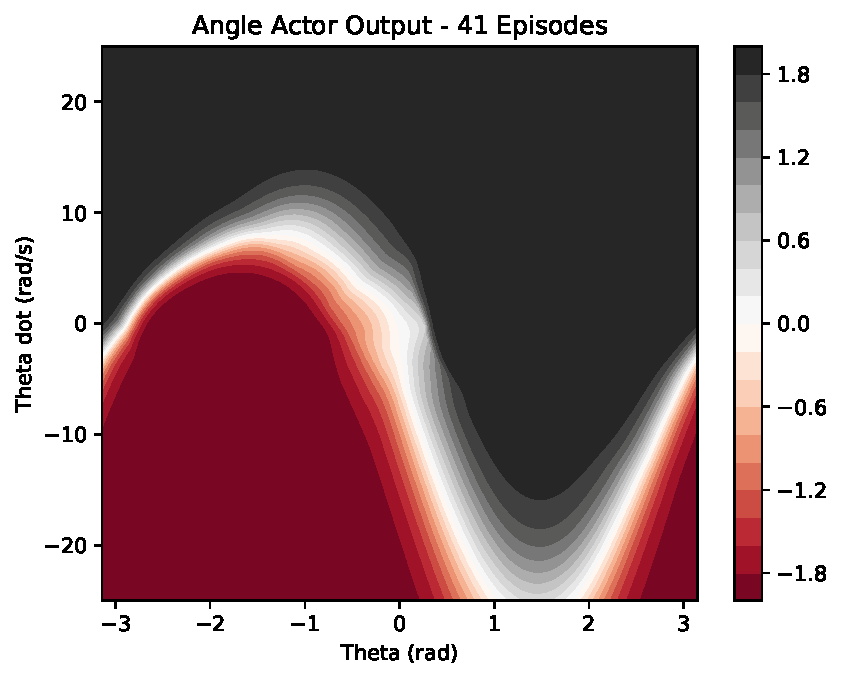
\includegraphics[width=65mm]{figures/train_figs/angle_actor/Actor0_41.pdf} &   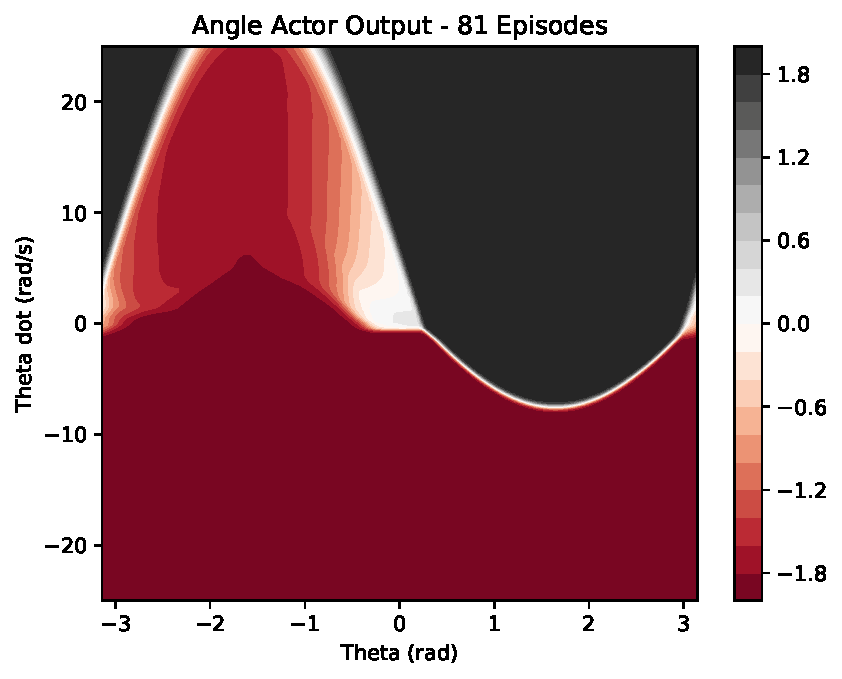
\includegraphics[width=65mm]{figures/train_figs/angle_actor/Actor0_81.pdf} \\
		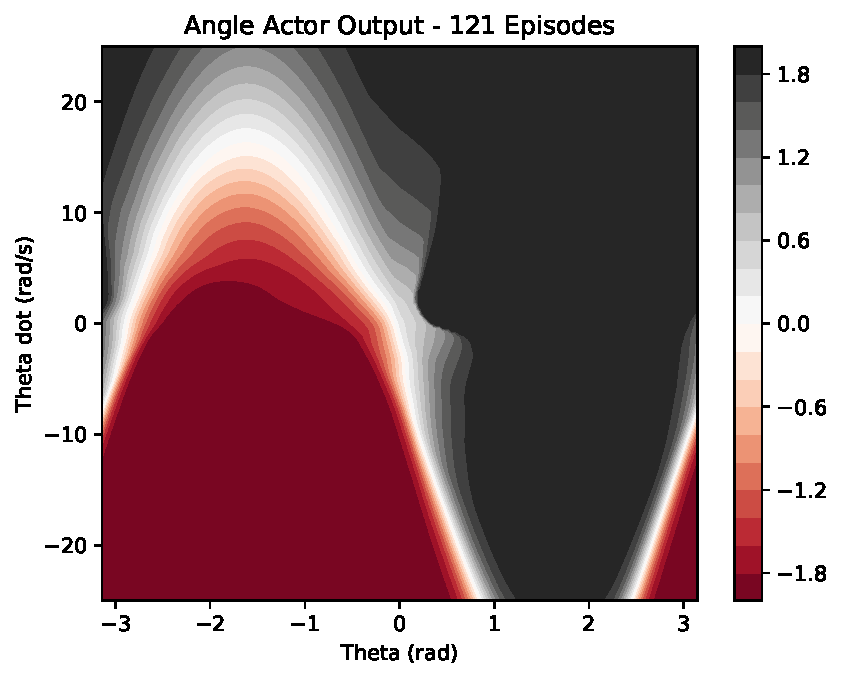
\includegraphics[width=65mm]{figures/train_figs/angle_actor/Actor0_121.pdf} &   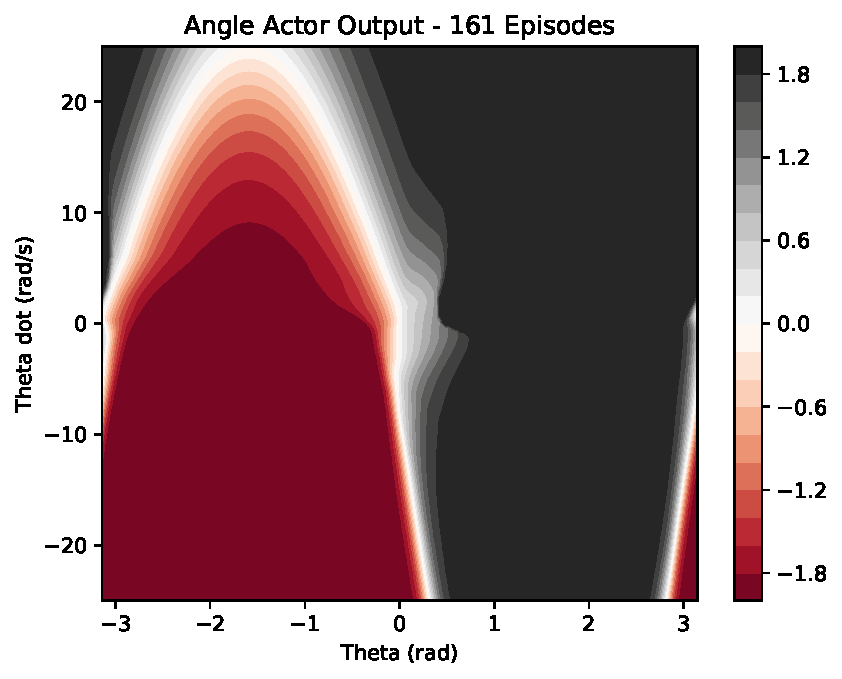
\includegraphics[width=65mm]{figures/train_figs/angle_actor/Actor0_161.pdf} \\
		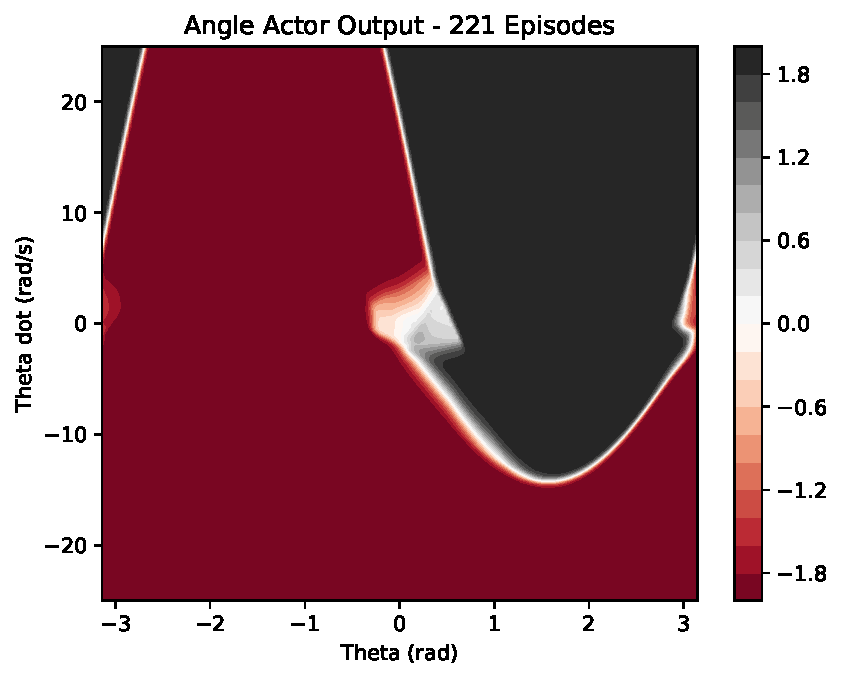
\includegraphics[width=65mm]{figures/train_figs/angle_actor/Actor0_221.pdf} &   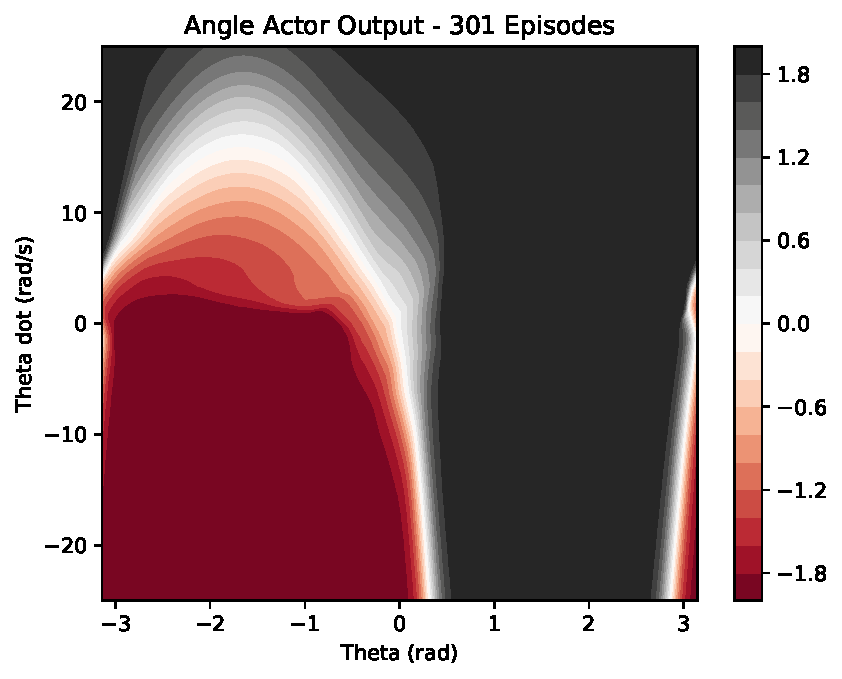
\includegraphics[width=65mm]{figures/train_figs/angle_actor/Actor0_301.pdf} \\
	\end{tabular}
	\caption{Angle Actor Output Progression}\label{fig:angle_actor_contour}
\end{figure}
\begin{figure}[H]
	\begin{tabular}{cc}
		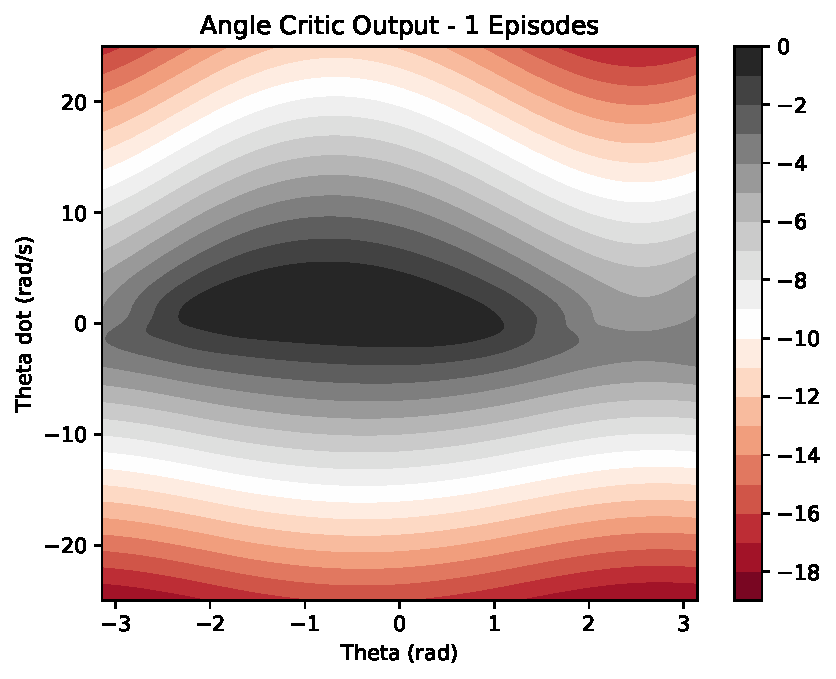
\includegraphics[width=65mm]{figures/train_figs/angle_critic/Critic0_1.pdf} &  
		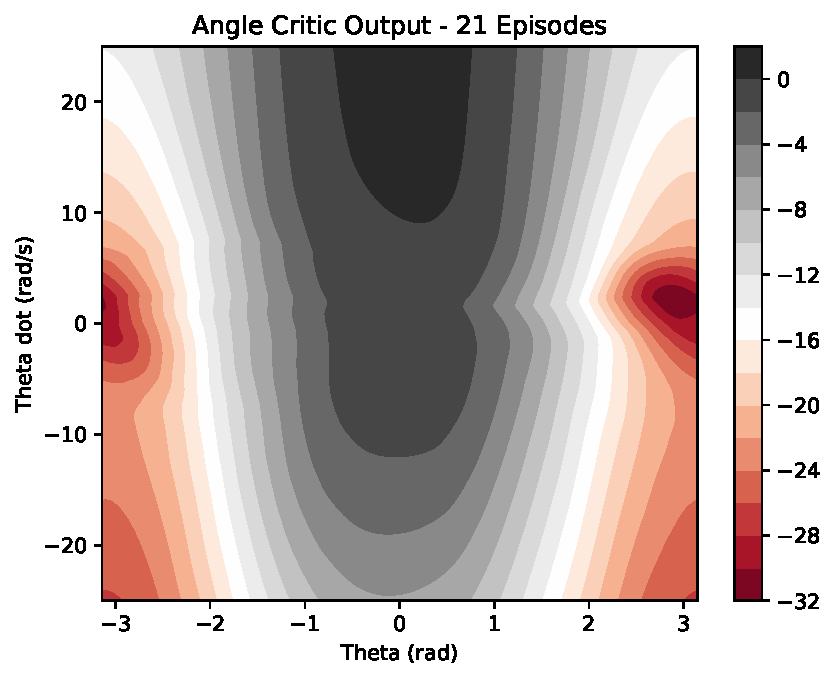
\includegraphics[width=65mm]{figures/train_figs/angle_critic/Critic0_21.pdf} \\
		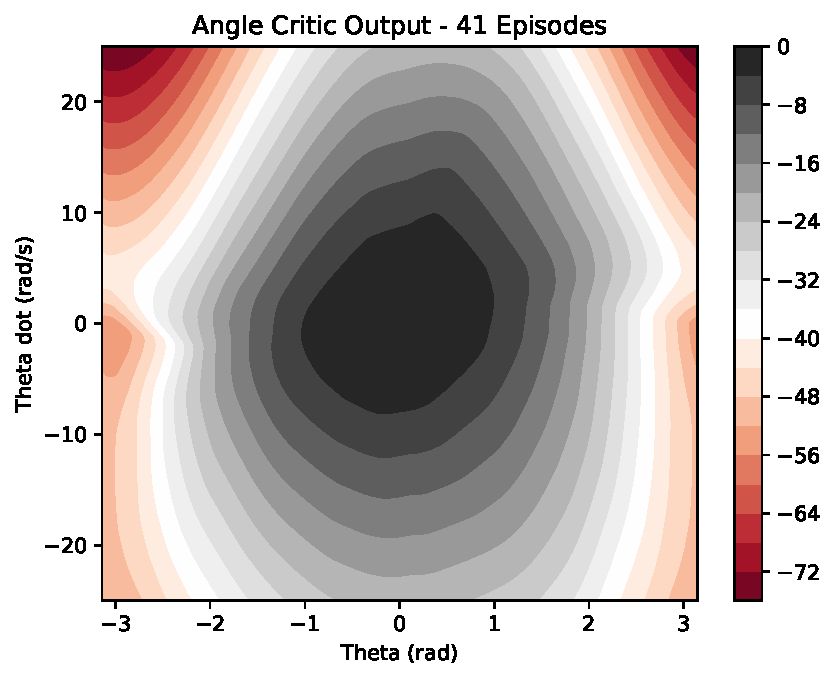
\includegraphics[width=65mm]{figures/train_figs/angle_critic/Critic0_41.pdf} &   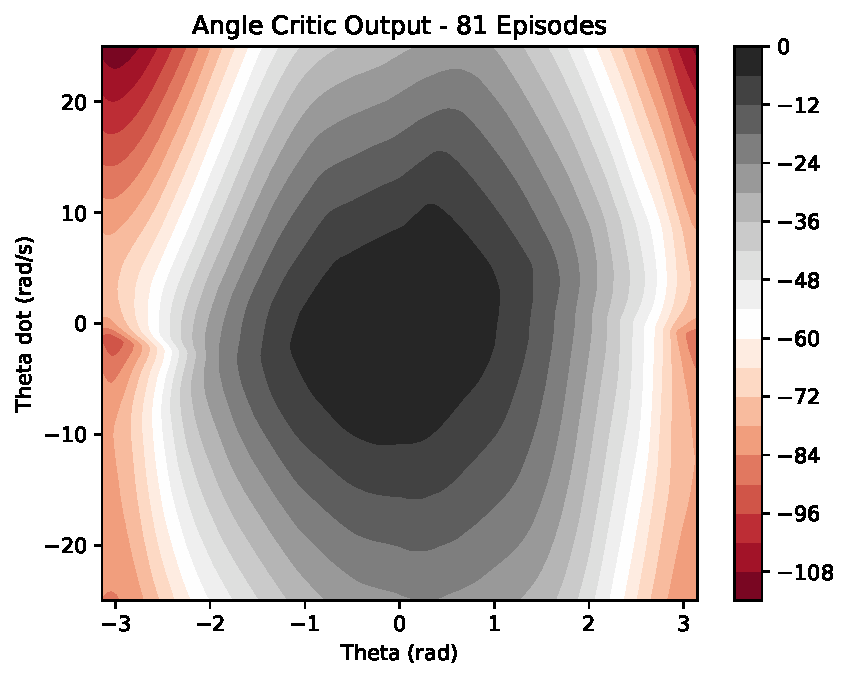
\includegraphics[width=65mm]{figures/train_figs/angle_critic/Critic0_81.pdf} \\
		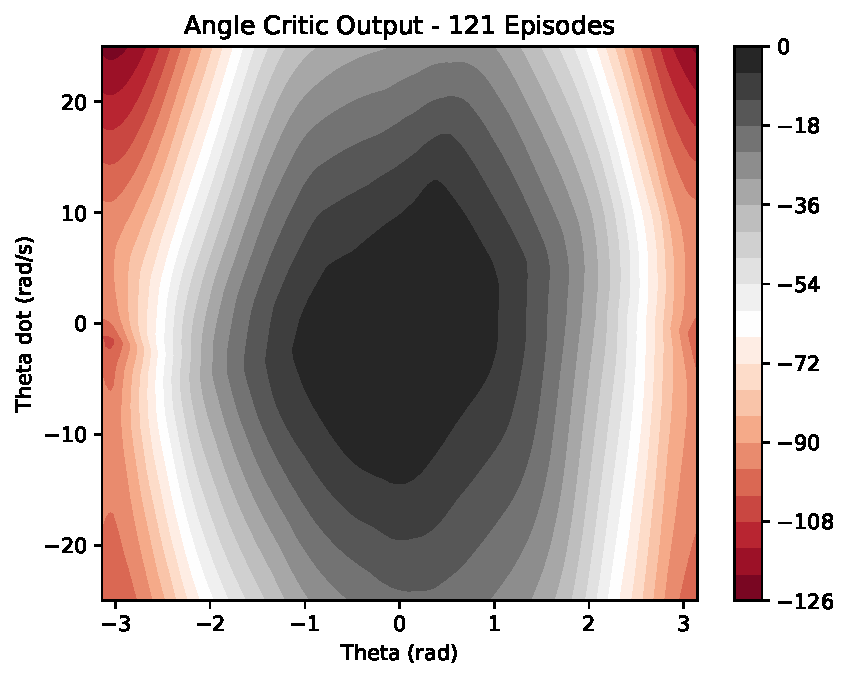
\includegraphics[width=65mm]{figures/train_figs/angle_critic/Critic0_121.pdf} &   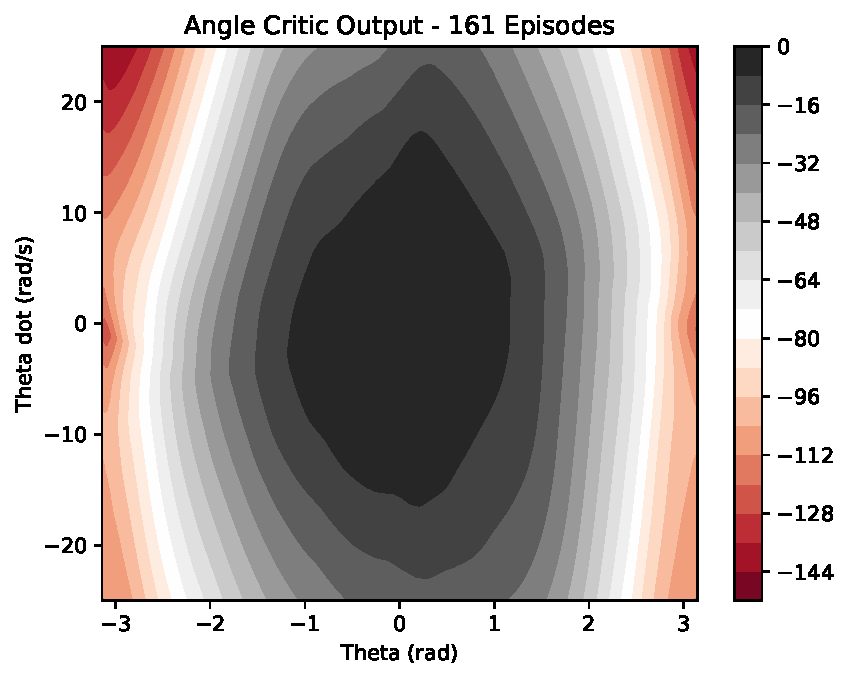
\includegraphics[width=65mm]{figures/train_figs/angle_critic/Critic0_161.pdf} \\
		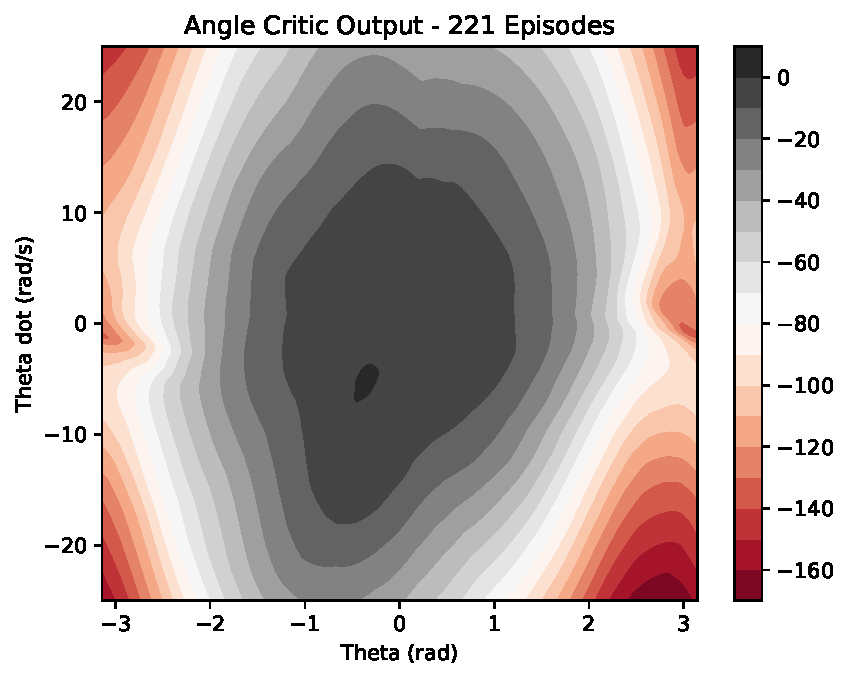
\includegraphics[width=65mm]{figures/train_figs/angle_critic/Critic0_221.pdf} &   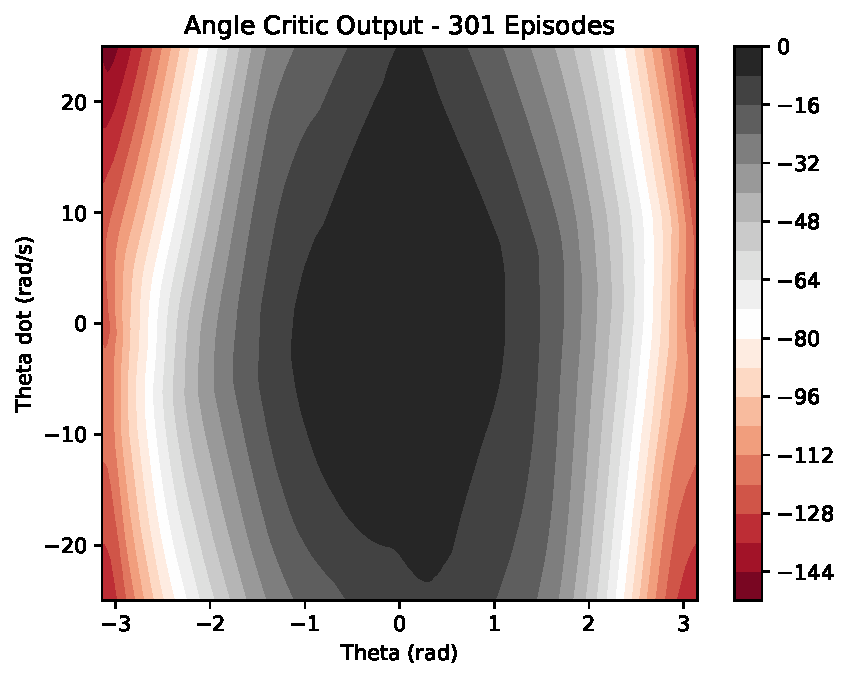
\includegraphics[width=65mm]{figures/train_figs/angle_critic/Critic0_301.pdf} \\
	\end{tabular}
	\caption{Angle Critic Output Progression}\label{fig:angle_critic_contour}
\end{figure}

\subsection{Single Actor Variant}
\begin{figure}[H]
	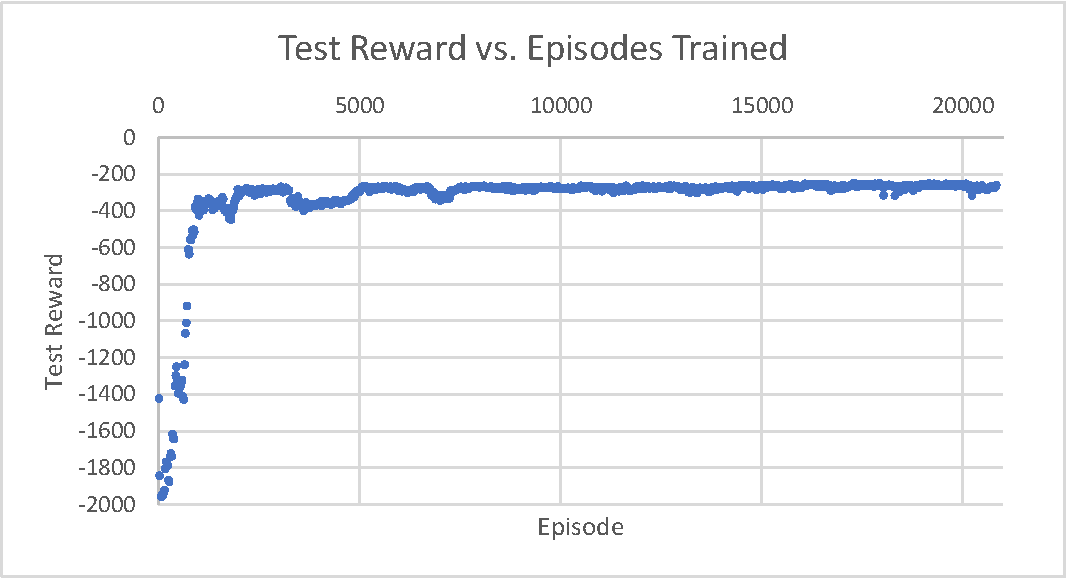
\includegraphics[width=6in, height=3.85in, keepaspectratio]{figures/train_figs/all_r.pdf}
	\caption{Training and Test Reward} \label{fig:all_r}
\end{figure}
\begin{figure}[H]
	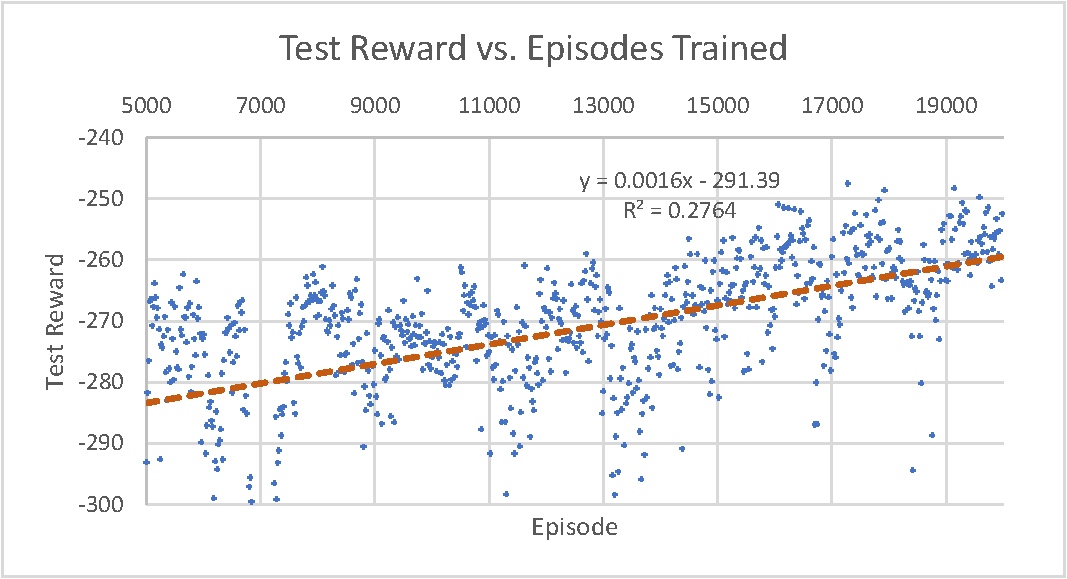
\includegraphics[width=6in, height=3.85in, keepaspectratio]{figures/train_figs/all_rzoom.pdf}
	\caption{Training and Test Reward Zoomed} \label{fig:all_rzoom}
\end{figure}
\begin{figure}[H]
	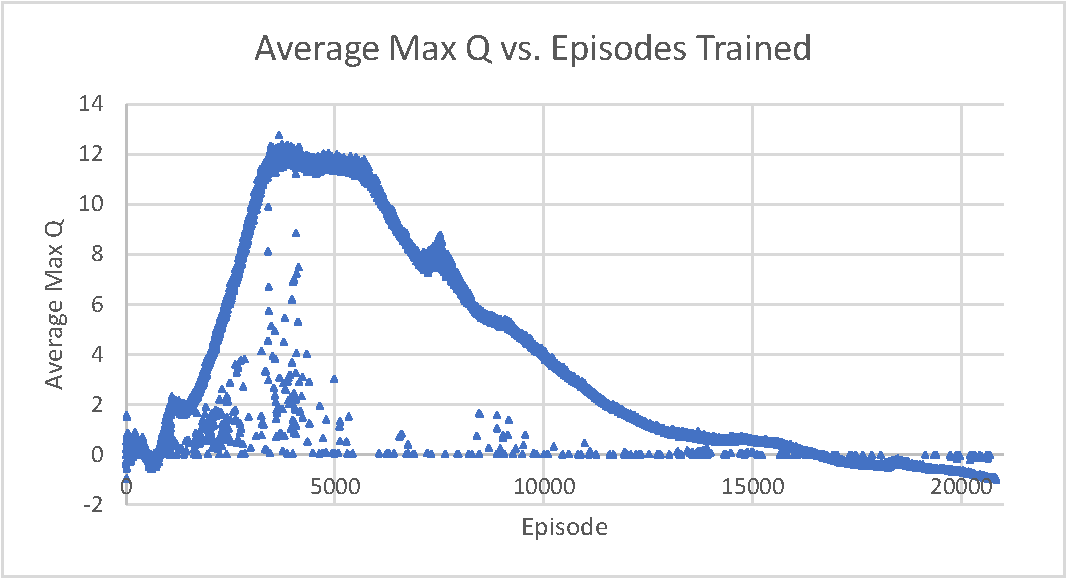
\includegraphics[width=6in, height=3.85in, keepaspectratio]{figures/train_figs/all_q.pdf}
	\caption{Average Max Q} \label{fig:all_q}
\end{figure}

\begin{figure}[H]
	\centering
	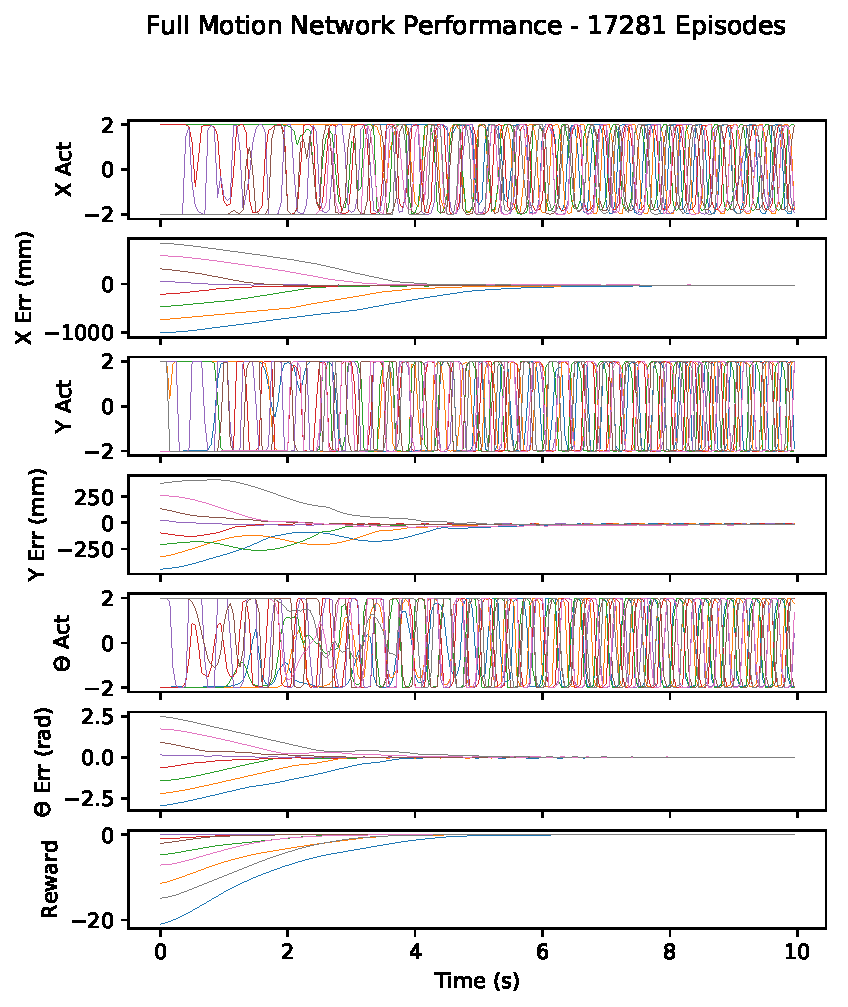
\includegraphics[width=6in,  keepaspectratio]{figures/train_figs/all_transitions/3_17281.pdf}
	\caption{All Network Performance -- 17281 Episodes}\label{fig:all_perf}
\end{figure}